During the dedicated experiment that took place in the SPS
in 2018 with the CCs, the measured emittance
growth was found to be a factor of four (on average) lower than
expected from the theory (see Section~\ref{sec:meas_2018_vs_theory}). The reason for this discrepancy remained unresolved for some time, as detailed follow-up studies (see Chapter~\ref{Ch:investigating_discrepancy}) investigated and excluded a number of possible explanations for the discrepancy.
It was recently found, that the beam transverse impedance, which is not included in the theory~\cite{PhysRevSTAB.18.101001} used for the comparison with the measurements may impact the noise-induced emittance growth and explain the experimental observations. Here, the damping mechanism from the beam transverse impedance is investigated as observed in detailed PyHEADTAIL simulations.

The structure of this chapter is as follows: Section~\ref{sec:sps_impedance_model} provides information on the impedance model of the SPS machine and benchmarks its implementation in PyHEADTAIL against theoretical calculations. In Section~\ref{sec:setup_simulations_emit_growth} the simulation setup for the emittance growth studies is discussed and the beam and machine parameters (following the 2018 $\CC$ experiment) are listed. Section~\ref{sec:first_obs_suppression} presents simulations results which showed for the first time that the transverse beam impedance (which was not included in the theory~\cite{PhysRevSTAB.18.101001} and the simulations up to now) significantly suppresses the noise-driven emittance growth. Thereafter, multiple PyHEADTAIL simulations were carried out aiming to characterise the effect of the suppression in order to understand the mechanism behind it. These studies are presented in Section~\ref{sec:emittance_growth_exploratory_studies}. The suppression mechanism is investigated through parametric studies and with studies in the frequency domain in Section~\ref{sec:suppression_mechanism}. Finally, the main results are summarised in Section~\ref{sec:Ch7_conclusions}


\section{SPS transverse impedance model}\label{sec:sps_impedance_model}
The PyHEADTAIL studies presented in this chapter are performed including the detailed transverse impedance model of the SPS machine~\cite{sps_impedance_model_git}. This model has been developed through a combination of theoretical computations and electromagnetic simulations and was benchmarked with beam-based measurements~\cite{Salvant:1274254, Zannini:1561199, Salvant:1271349, Zannini:2141779}. 
It includes the contributions from all the individual elements in the SPS lattice i.e. the resistive wall, the indirect space charge, the kickers, the RF cavities (200\,MHz and 800\,MHz), the step transitions, and the horizontal and vertical beam position monitors~\cite{Zannini:2141779}. As discussed in  Section~\ref{subsec:pyheadtail}, the model needs to represent the global impedance of the full machine. Thus, the total impedance is obtained by summing up the impedance of each element weighted with the beta function at its location and by dividing the sum by the average beta function of the SPS. For the Q26 optics, the average horizontal and vertical beta functions are 42.09\,m, and 42.01\,m respectively.
%https://indico.cern.ch/event/299470/contributions/686509/attachments/564150/777102/LIUSPS_transverse_imp_5.pdf
% The Wall contribution included both the resistive wall and the indirect SC.
Figure~\ref{fig:sps_impedance_model_H_V} shows the complete transverse impedance model of the SPS machine with the disentangled dipolar (blue) and quadrupolar (orange) terms to be plotted seperetaly. 

% Plot figures: /eos/user/n/natriant/Project_thesis/plot_wakefields_impedances_SPS
\begin{figure}[!ht]
    \centering
    \begin{subfigure}[t]{0.45\textwidth}
        \centering
        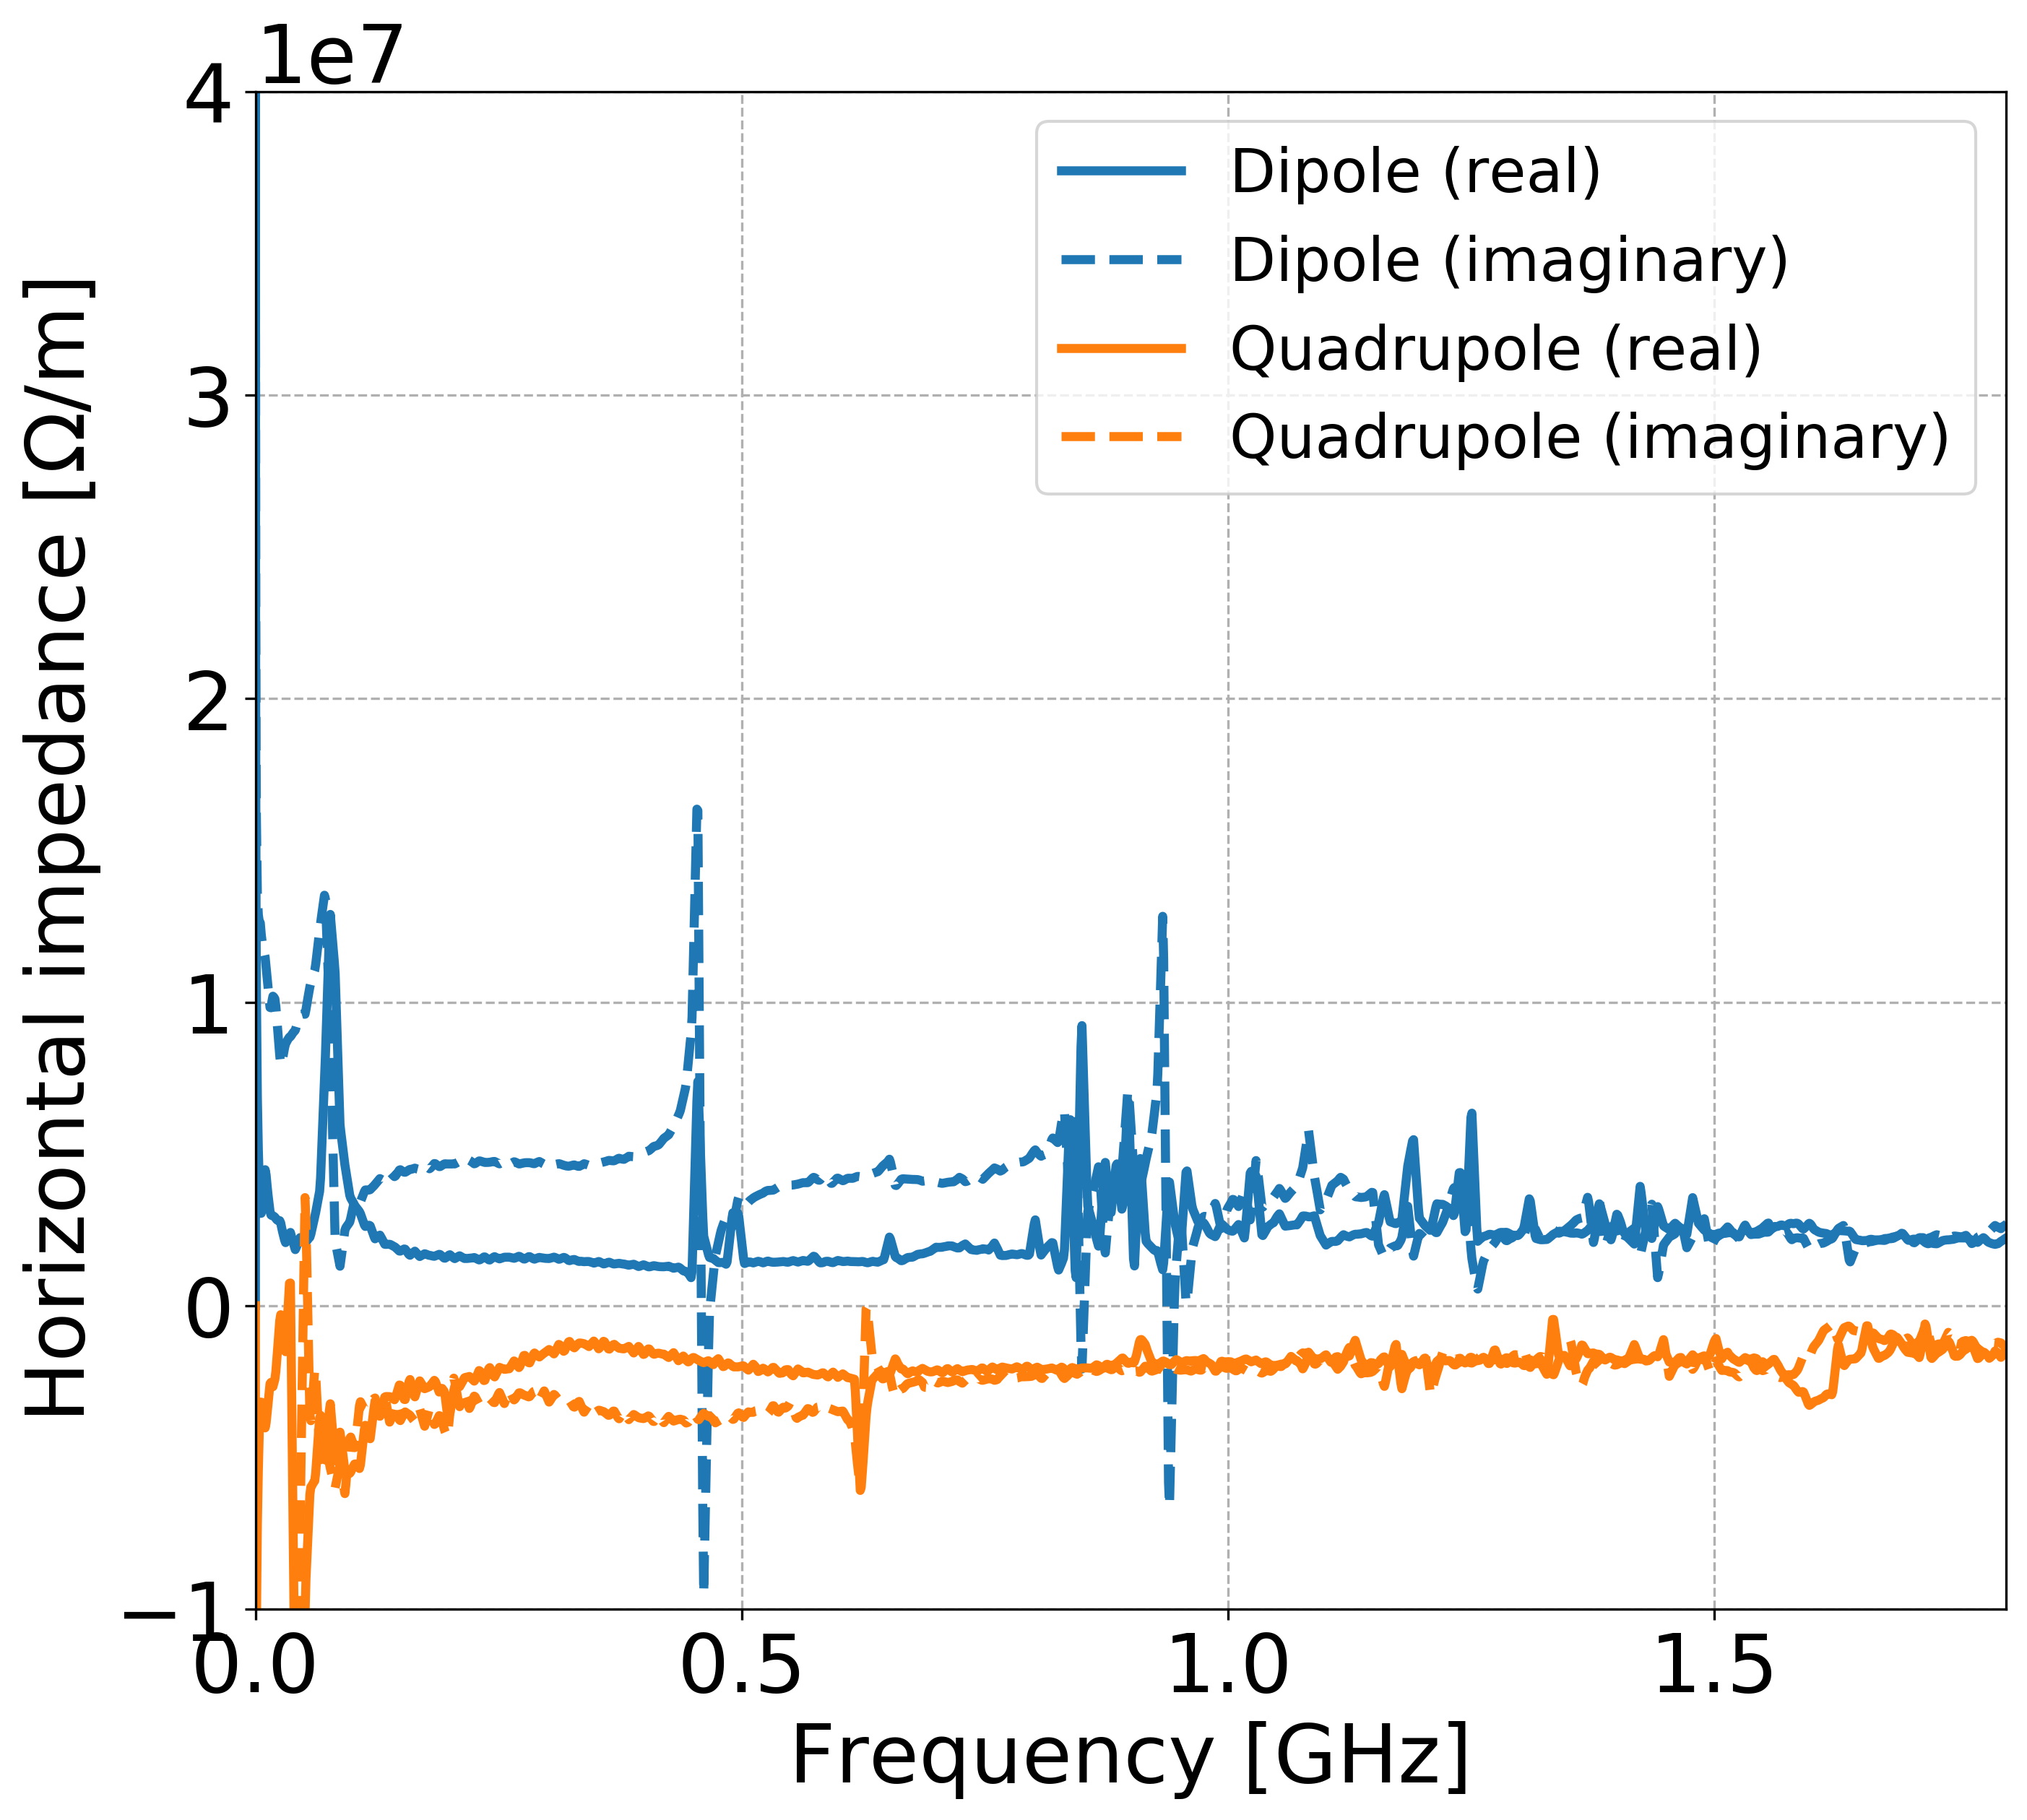
\includegraphics[width=1\textwidth]{images/Ch7/Q26_complete_SPS_model_impedance_H_plane.png}
        %\caption{$y=\sin(2 \pi f t),\ f=50$ Hz}
        %\label{fig:add_label_here}
    \end{subfigure}
    \hfill
    \begin{subfigure}[t]{0.45\textwidth}
        \centering
        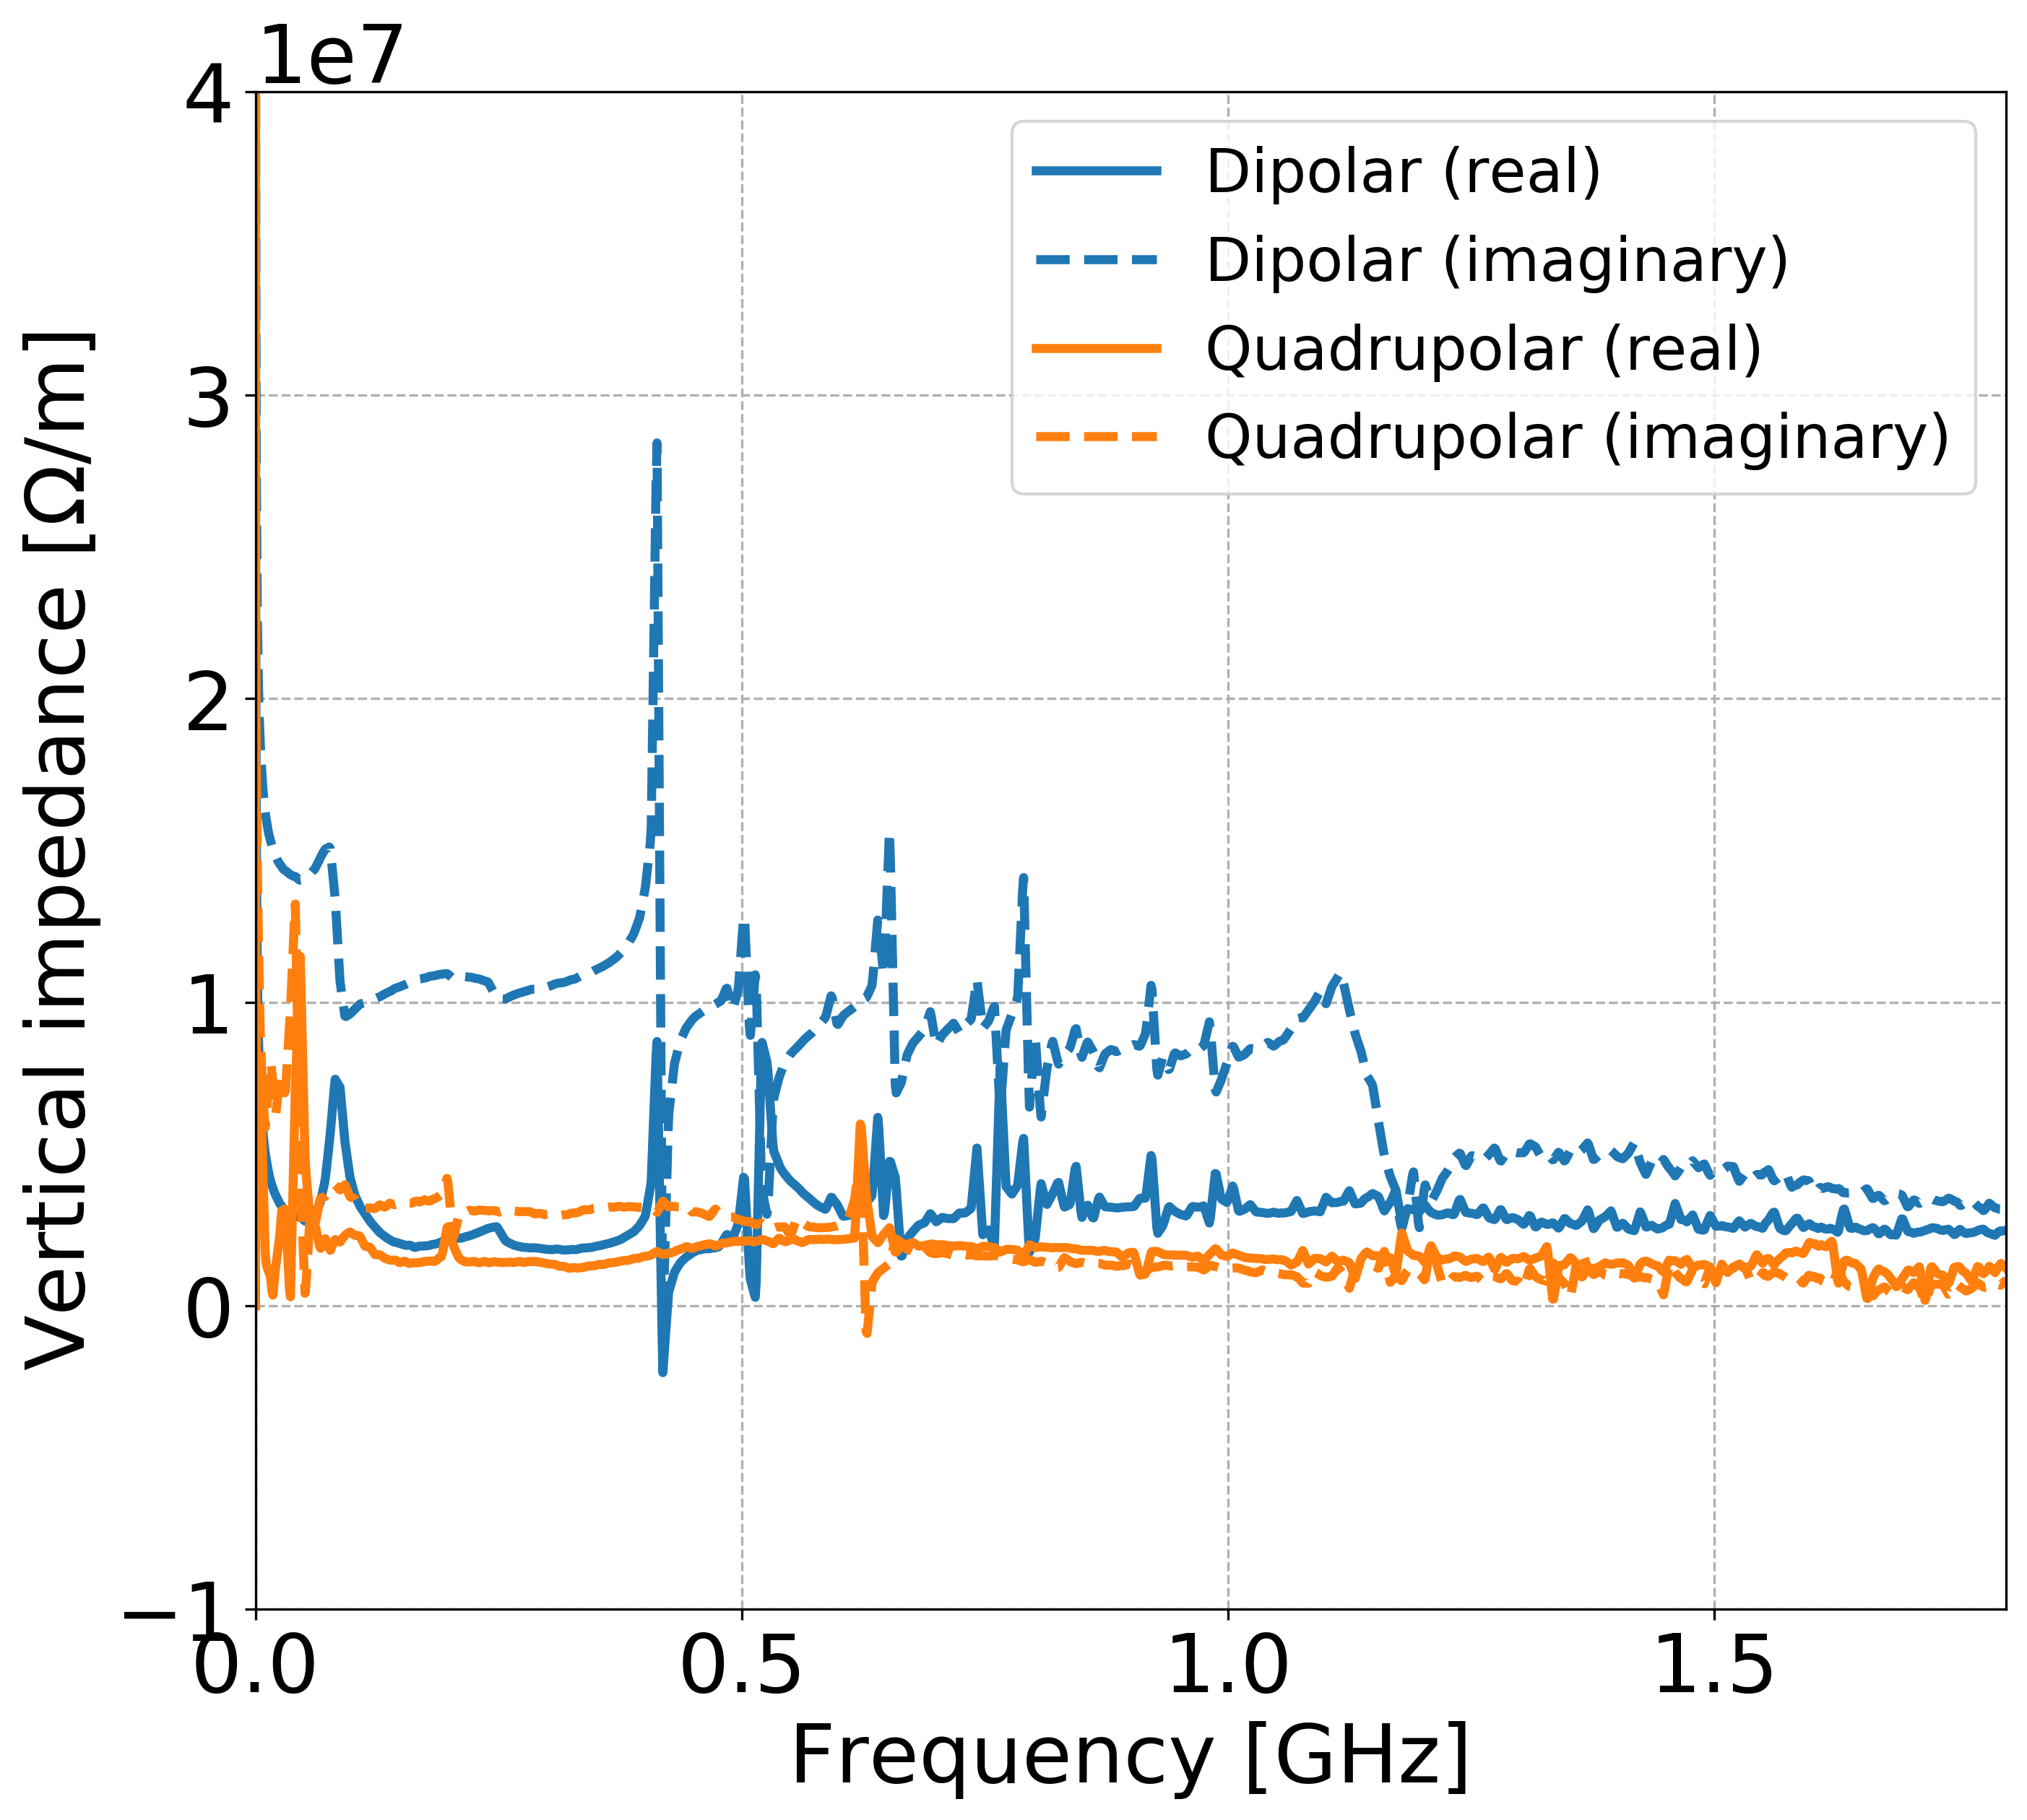
\includegraphics[width=1\textwidth]{images/Ch7/Q26_complete_SPS_model_impedance_V_plane.png}
        %\caption{Discrete Fourier transform}
        %\label{fig:add_label_here}
    \end{subfigure}
    \hfill
     \caption{Horizontal (left) and vertical (right) impedance model of the SPS. The model is available in the public GitLab repository of Ref.~\cite{sps_impedance_model_git}.} % bunch passage
     \label{fig:sps_impedance_model_H_V}
 \end{figure}

 The contributions from the wall, the kickers and the step transitions are visible at the low freqencies (up to $\sim$ 0.4\,GHz). The impedance of the RF cavities and the beam position monitors (BPMs) corresponds results to the peaks observed between $\sim$ 0.4-1\,GHz. 
%https://indico.cern.ch/event/299470/contributions/686509/attachments/564150/777102/LIUSPS_transverse_imp_5.pdf %For a clearer picture, it is worth mentioning that at low freqencies (up to $\sim$ 0.4\,GHz) the impedance is mainly from the wall the kickers and the step transitions. The peaks between $\sim$ 0.4-1\,GHz appear due to the RF cavities and the beam position monitors.
%https://indico.cern.ch/event/299470/contributions/686509/attachments/564150/777102/LIUSPS_transverse_imp_5.pdf


\normalsize{\textbf{Wake functions}}\\
As already discussed in Section~\ref{subsec:pyheadtail}, in order to include the impedance effects in PyHEADTAIL simulations the real-value wakefields in the time domain are used. The wakefield kicks are computed as a convolution of the wake function with the moments of each particle. The total transverse dipolar (blue) and quadrupolar (orange) wake functions for both planes of the SPS can be found in the GitLab repository of Ref.~\cite{sps_impedance_model_git} and they are plotted in Fig~\ref{fig:sps_wakefunctions_model_H_V}.

% Plot figures: /eos/user/n/natriant/Project_thesis/plot_wakefields_impedances_SPS
 \begin{figure}[!ht]
    \centering
    \begin{subfigure}[t]{0.45\textwidth}
        \centering
        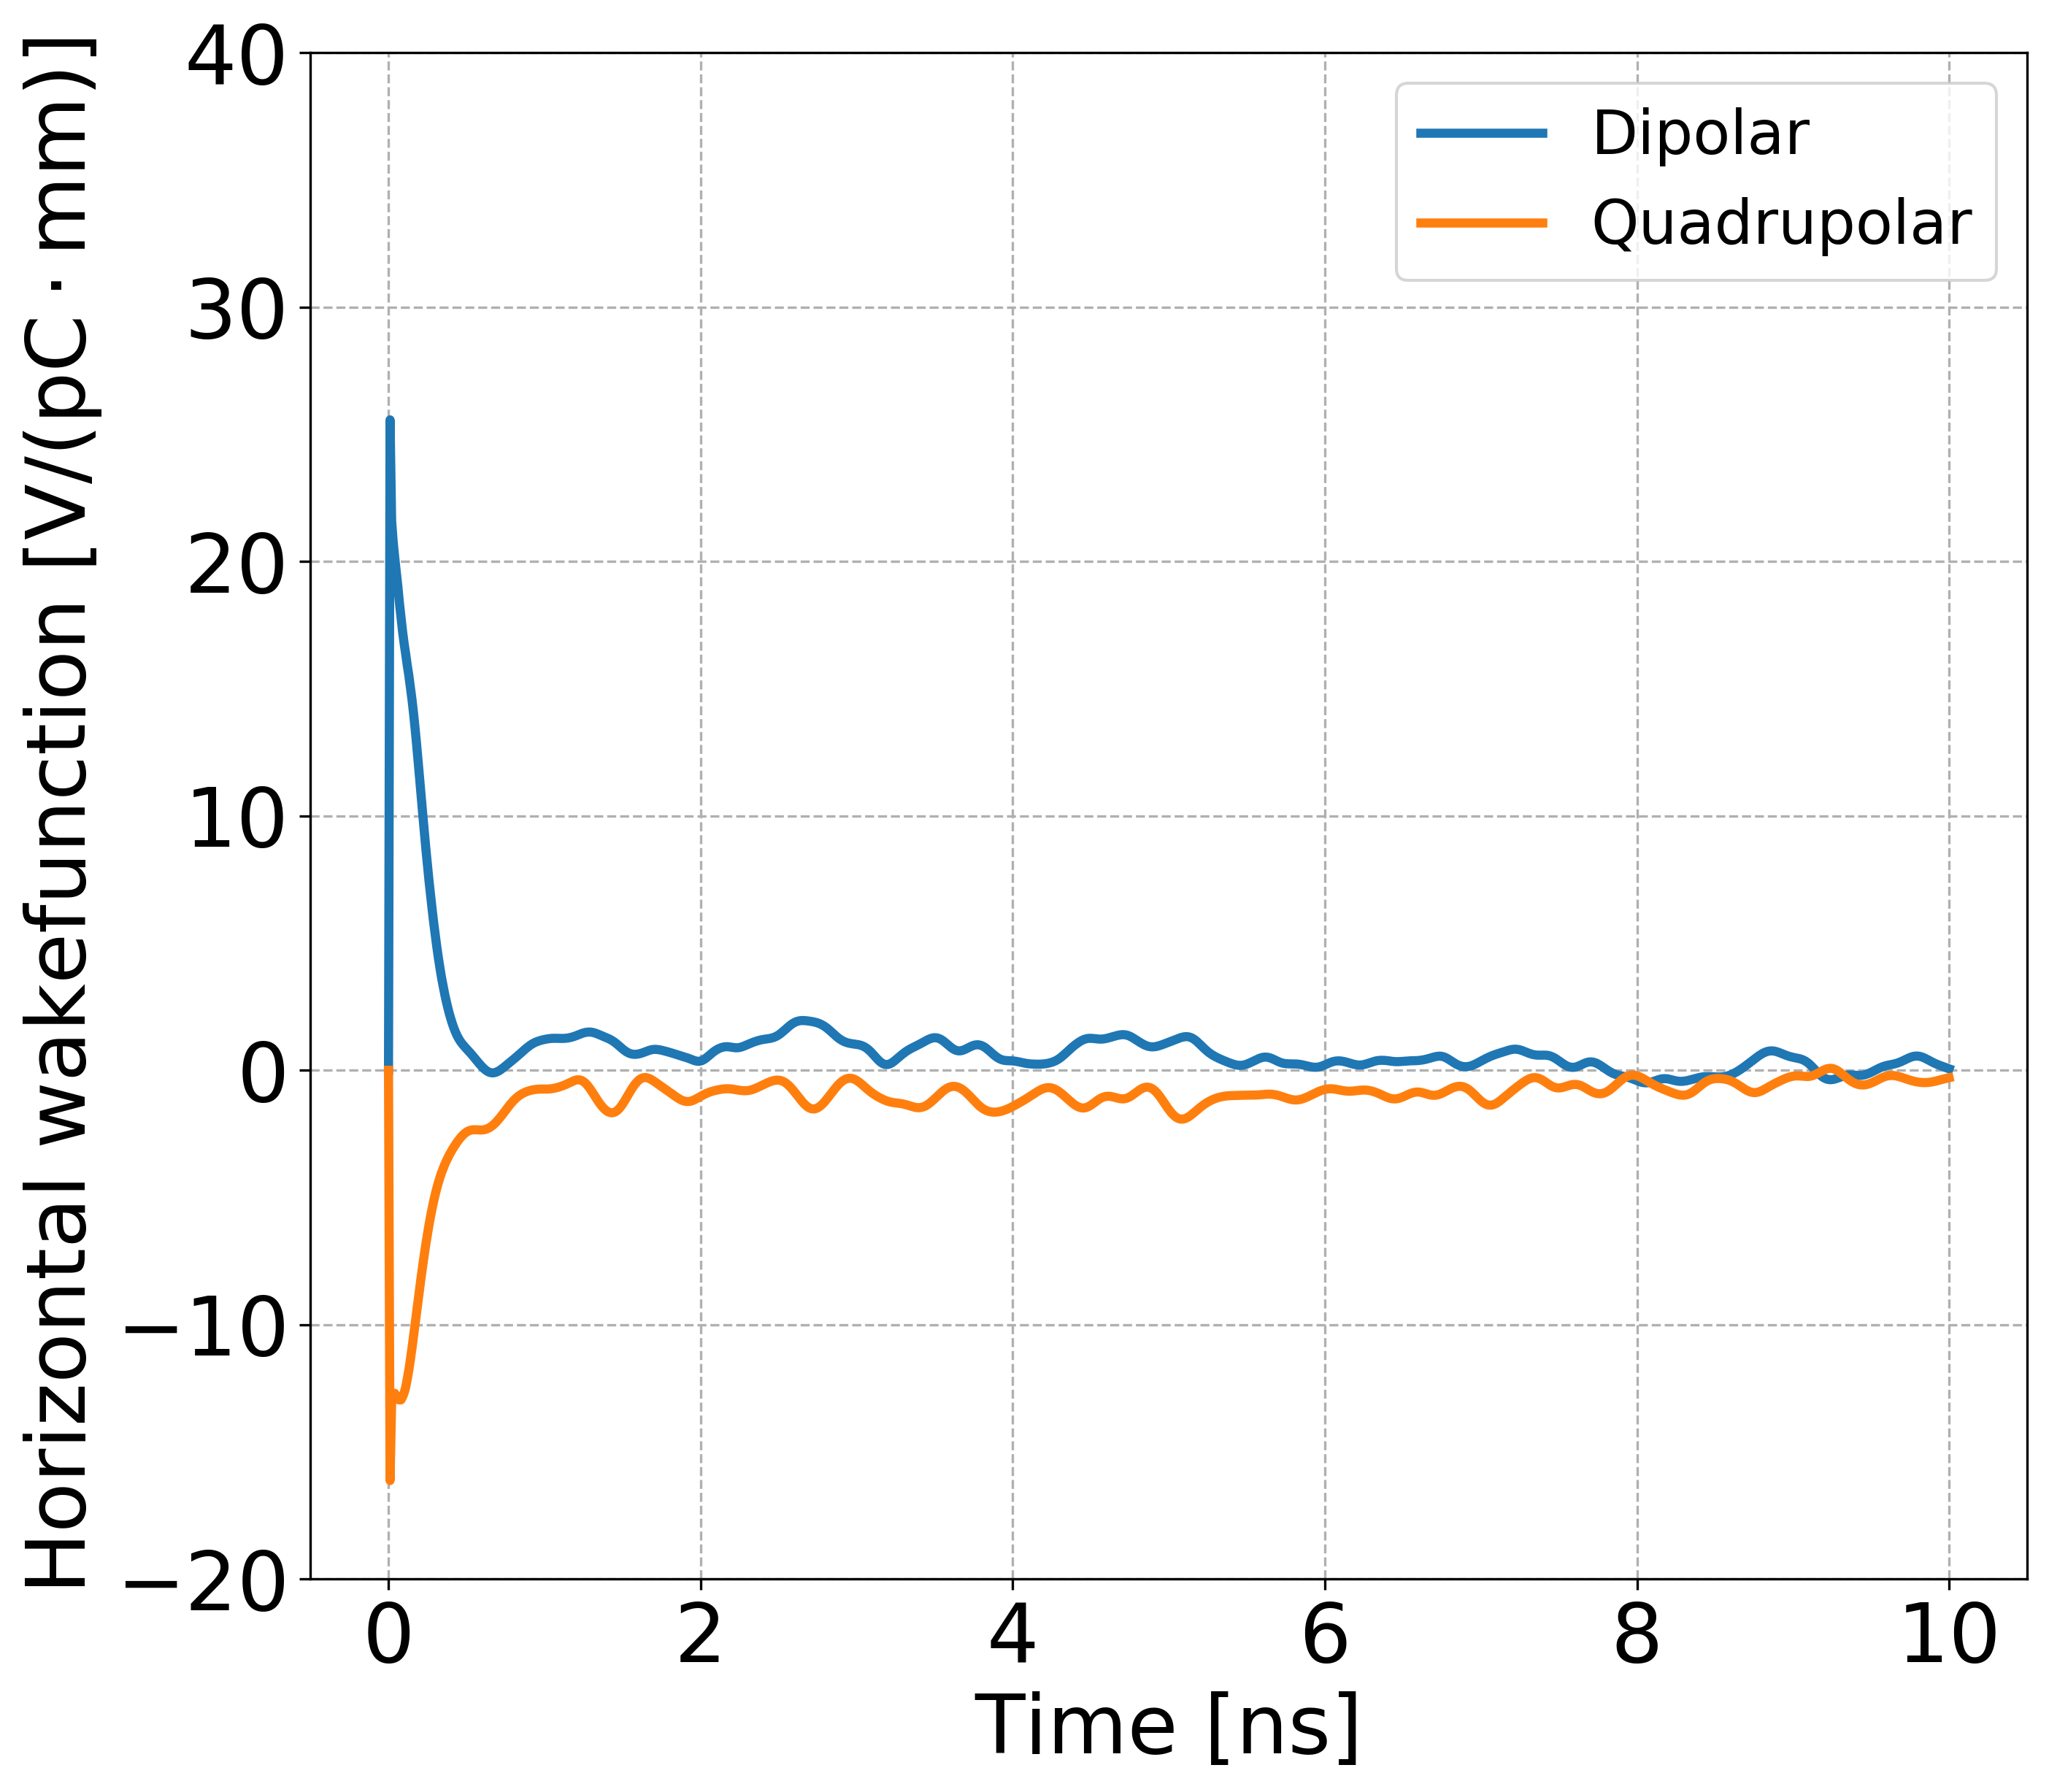
\includegraphics[width=1\textwidth]{images/Ch7/Q26_complete_SPS_model_wakefunctions_H_plane.png}
        %\caption{$y=\sin(2 \pi f t),\ f=50$ Hz}
        %\label{fig:add_label_here}
    \end{subfigure}
    \hfill
    \begin{subfigure}[t]{0.45\textwidth}
        \centering
        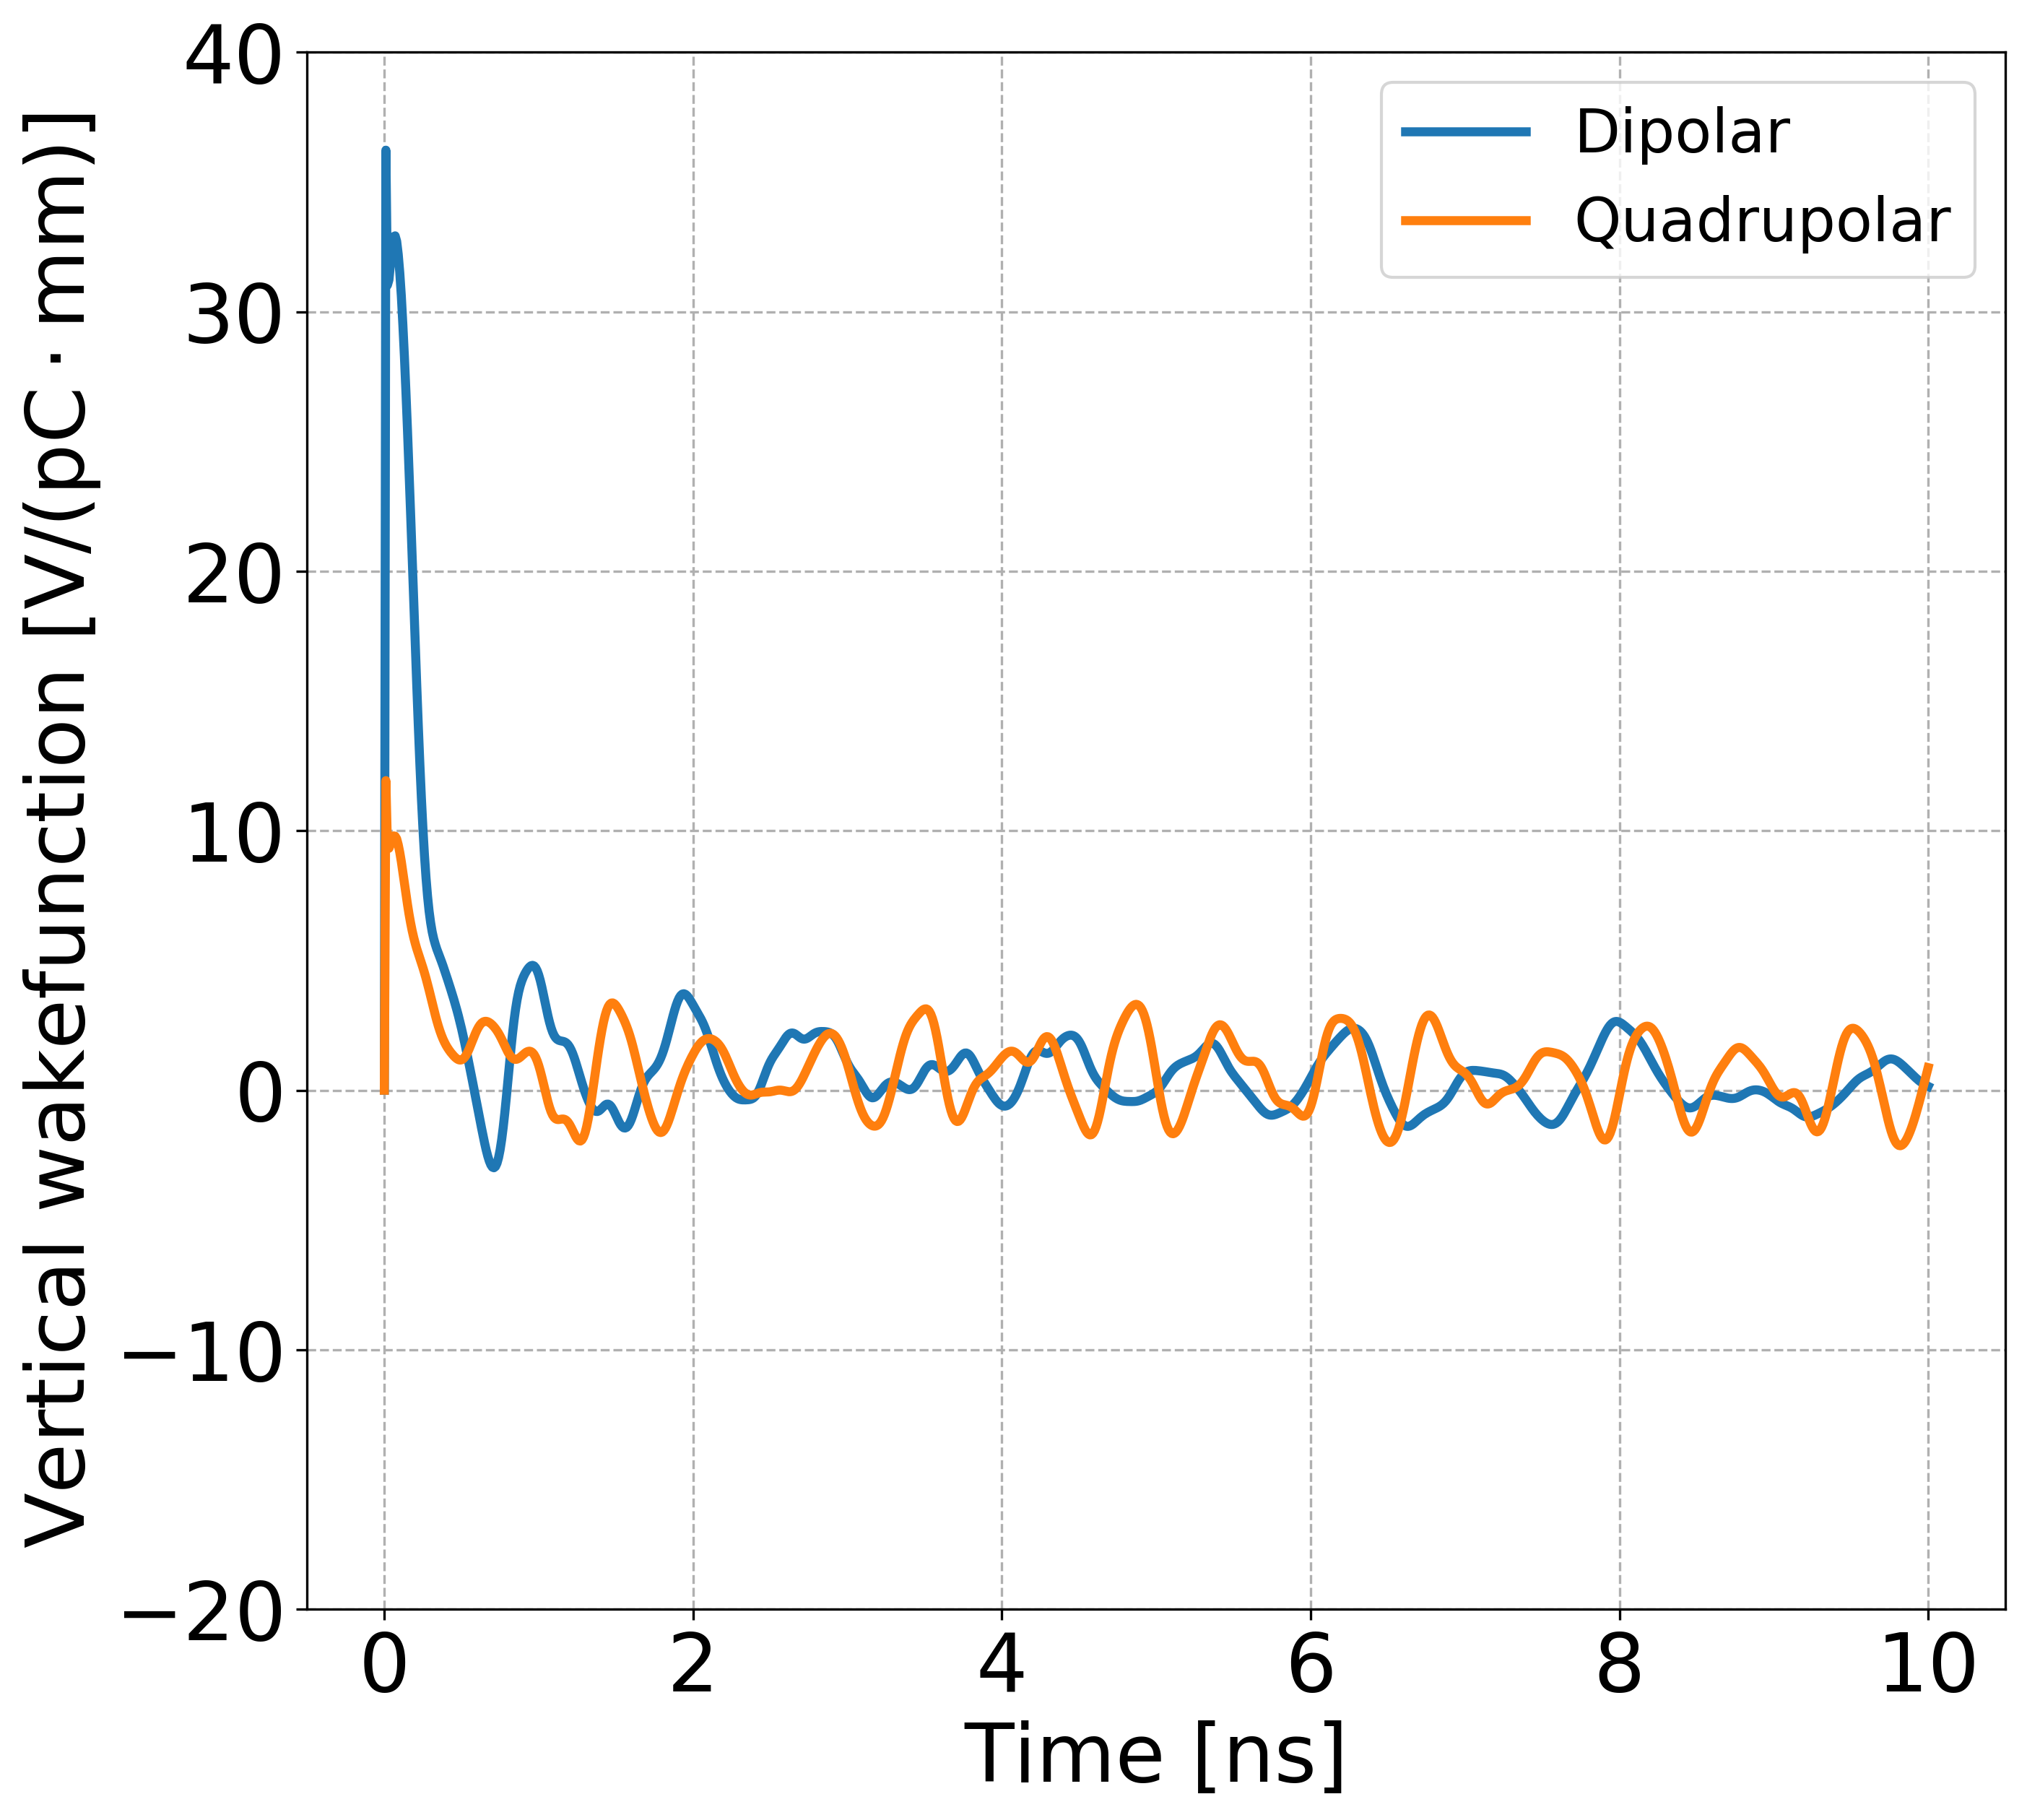
\includegraphics[width=1\textwidth]{images/Ch7/Q26_complete_SPS_model_wakefunctions_V_plane.png}
        %\caption{Discrete Fourier transform}
        %\label{fig:add_label_here}
    \end{subfigure}
    \hfill
     \caption{Horizontal (left) and vertical (right) wakefunctions of the SPS. The wake functions are available in the public GitLab repository of Ref.~\cite{sps_impedance_model_git}. For comparison the bunch length in the SPS CC experiments is $\sim$ 1.85\,ns (4$\mathrm{\sigma_t}$).} % bunch passage
     \label{fig:sps_wakefunctions_model_H_V}
 \end{figure}

The constant terms, in both transverse planes, equal zero in the SPS impedance model. The reason behind this, is that firstly the constant term is usually coming from asymmetries in the various structures which are not significant, and secondly, the constant term does not lead to instabilities or tune shift, so usually is not of big concern.

 For refernece, the impedance model is used as an input in the Sacherer formula (Eq.~\eqref{eq:complext_tune_shift_modes_m}) for analytical estimations while the wake functions are used as an input in simulation codes such as PyHEADTAIL.

Last, these wake functions are obtained with an inverse Fast Fourier Transform algorithm (iFFT) on the imepdance model as described in the references provided above.

% slide 9 https://accelconf.web.cern.ch/ipac2019/talks/weypls1_talk.pdf

% Carlo Zaninni thesis: s, it is important to have an accurate description of the wake at a distance z significantly smaller than the RMS bunch-length, which means that the impedance calculation needs to be accurate up to very high frequency (depending on the accelerator we consider, from a few GHz to the range of THz). 

\subsection{Testing the implementation in PyHEADTAIL}\label{subsec:test_implementation_pyheatail}
As discussed in Section~\ref{subsec:wakefields} the imaginary part of the impedance leads to a coherent tune shift which depends on the bunch intensity. One of the most common ways to test the correct implementation of the impedance model in a tracking simulation code is to benchmark the simulated intensity-dependent coherent tune shift with the theoretically predicted behavior (using Eqs.~\eqref{eq:complext_tune_shift_modes_m} and ~\eqref{eq:real_tunu_mode_l}).

Typically, in tracking simulations, the coherent tune is obtained by applying a frequency analysis technique to the oscillations of the centroid of the particle distribution (the center of mass of the bunch). Here, the analysis is limited to the coherent mode $l=0$ as it can be obtained using a simple Fast Fourier Transform (FFT) algorithm~\cite{FFT_and_applications}. Higher modes (in absolute value, i.e. $l=\pm 1, \pm 2$ etc) can be obtained with more complex algorithms such as the oned provided from the SUSSIX code~\cite{Bartolini:702438} \footnote{The SUSSIX code is applied to the complex position in phase space, $u-i p_u$, while an FFT algorithm is applied only to the transverse position $u$, where $u=(x,y)$~\cite{Salvant:1274254}.}. Nevertheless, the study of mode $l=0$ is sufficient for the purpose of the studies presented here. For simplicity in the following the term "coherent tune" will refer to the coherent tune of mode $l=0$.

\textbf{Simulations setup}\\
The parameters used for setting up the linear transfer map, the longitudinal tracking and the beam initialisation are shown in Table~\ref{tab:pyheadtail_simulation_parameters} and are the ones used in the SPS $\CC$ experiment of 2018. The ring is consisted of one segment, with one interaction point at which the beam interacts with the wakefields. At that location, the horizontal and vertical beta functions equal the corresponding average beta functions over the SPS machine (see Section~\ref{subsec:pyheadtail}). The latest transverse wakefield model (as of February 2019 in Ref.~\cite{sps_impedance_model_git}) of the SPS was used.

The initial bunch was generated with Gaussian distributions in transverse and longitudinal planes. The bunch population of the different intensity values was represented by $5 \times 10^5$ macroparticles and the number of slices of the longitudinal distribution was 500.

\begin{table}[!hbt]
	\begin{minipage}{\textwidth}
      \begin{centering}
   \caption{PyHEADTAIL simulation parameters used to study impedance induced effects for the SPS.}
	\begin{tabu} to \textwidth {X[c,m] X[0.5c,m] X[0.5c,m] X[0.01c,m]}
		&&& \\[-6mm]
		\toprule \toprule
		\multicolumn{2}{l}{\textbf{Parameter}} &
		\multicolumn{2}{c}{\textbf{Value}} \\
		\bottomrule
      \multicolumn{2}{l}{Beam energy, $\symE$} & \multicolumn{2}{c}{270\,GeV} \\
      \multicolumn{2}{l}{Machine circumference, $C_0$}  & \multicolumn{2}{c}{6911.5623\,kHz} \\
      \multicolumn{2}{l}{Horizontal / Vertical betatron tune, $\Qx$ / $\Qy$}  & \multicolumn{2}{c}{26.13 / 26.18} \\
      \multicolumn{2}{l}{Synchrotron tune, $\Qs$}  & \multicolumn{2}{c}{0.0051}\\
      \multicolumn{2}{l}{Momentum compaction factor, $\alpha_p$}  & \multicolumn{2}{c}{1.9 $\times 10^{-3}$}\\
      \multicolumn{2}{l}{Number of bunches}  & \multicolumn{2}{c}{1} \\
      \multicolumn{2}{l}{Rms bunch length, 4$\sigmat$}  & \multicolumn{2}{c}{1.7\,ns $^\ast$}\\
      \multicolumn{2}{l}{Horizontal / Vertical normalised emittance, $\epsilon_x$ / $\epsilon_y$}  & \multicolumn{2}{c}{2\,$\mathrm{\mu m}$ / 2\,$\mathrm{\mu m}$}\\
      \multicolumn{2}{l}{Average horizontal / vertical beta function, $\langle \beta_x \rangle / \langle \beta_y \rangle$}  & \multicolumn{2}{c}{42.0941\,m / 42.0137\,m $^\dagger$ } \\
      \bottomrule
      \multicolumn{2}{l}{Number of macroparticles, $N_\mathrm{mp}$}  & \multicolumn{2}{c}{$5 \times 10^5$} \\
      \multicolumn{2}{l}{Number of longitudinal slices, $N_\mathrm{slices}$}  & \multicolumn{2}{c}{500} \\
      \bottomrule
	\end{tabu}
   \label{tab:pyheadtail_simulation_parameters}
   \end{centering}\footnotesize{$^\ast$ This value corresponds to the average rms measured bunch length of bunch 1 over all the coasts of 2018. The value for bunch 1 is used here since it was the only stable bunch in the SPS $\CC$ tests of 2018. \\ $^\dagger$ Model values for the Q26 optics.}
   \end{minipage}
\end{table}
% 4 sigma_t = 1.7 in: cernbox/2018/CC_MD_2018_summary/ABWLM/bunch_length_pickle_file

For all the PyHEADTAIL simulation studies presented in this thesis, the Twiss parameter $\alpha_u(s)$ and the dispersion function $D_u(s)$ equal zero. This is a valid assumption for the studies as these parameters have no direct impact on the effects under investigation.

To facilitate the observation of the coherent tune, the bunch was intialised with a static offset of 0.15$\sigma_{x,y}$ in both transverse planes\footnote{The rms transverse beam size at the only interaction point along the ring i.e. at the location where the beam interacts with the wakefields.}, such as it performs dipole oscillations around the machine. Then, it was tracked for 600 turns and the coherent tune was computed using a NAFF algorithm~\cite{LASKAR1990266, Kostoglou:2289645}, which provides a refined FFT analysis, and its python implementation, NAFFlib, can be found in the corresponding package in Ref.~\cite{nafflib_repository}, on the turn-by-turn centroid motion. The coherent tune shift was computed by subtracting the obtained tune value from the unperturbed coherent tune (in the absence of impedance) which equals the $Q_{u0}$ value.

Last, the dependence of the coherent tune on the intensity value was studied in the absence of other detuning effects (such as chromaticity or detuning with transverse amplitude, even though they mainly introduce incoherent tune shifts). % Do they also introduce some small coherent tune?

The simulation was repeated for a range of bunch intensities, $N_b$, equally-spaced from 0 to $5 \times 10^{10}$ protons per bunch. This range was chosen to be in the vicinity of the bunch intensity of the $\CC$ experiments of 2018, where $N_b$ was $3\times 10^{10}$ protons per bunch. $N_b=0$ is not a realistic value. However, it is used here as the reference point for which the coherent betatron tune equals zero. The simulation results are plotted against the theoretically expected tune shifts in Fig.~\ref{fig:sps_coherent_DQ_vs_intensity_original_complete_model}.

The theoretically expected values are computed from Eqs.~\eqref{eq:complext_tune_shift_modes_m} and ~\eqref{eq:real_tunu_mode_l} for $l=0$ and using only the imaginary part of the imepdance. Given that $\Gamma(1/2)=\sqrt{\pi}$ and $Q_u = \omega_{u0}/\omega_\mathrm{rev}$ equation Eq.~\eqref{eq:complext_tune_shift_modes_m} becomes:
\begin{equation}\label{eq:real_tune_shfit_for_coherent_mode}
    \Delta \Omega_u^{(0)} =  \Omega_{u0}^{(0)} - \omega_{u0} = \frac{\sqrt{\pi}}{4 \pi}\frac{N_b r_0 c^2}{\gamma_0 \frac{2\pi}{\omega_\mathrm{rev}}\omega_u \sigma_z} Z_\mathrm{eff, im} = \frac{N_b r_0 c^2}{8 \pi^{3/2} \gamma_0 Q_u \sigma z}Z_\mathrm{eff, im}
\end{equation}
All the parameters inserted in Eq.~\eqref{eq:real_tune_shfit_for_coherent_mode} should be converted in CGS (centimetre–gram–second) units.

Then the coherent betatron tune shift is computed by inserting the result of Eq.~\eqref{eq:real_tune_shfit_for_coherent_mode} in Eq.~\eqref{eq:real_tunu_mode_l} such as 
\begin{equation}
    \Delta Q_u = \frac{\Delta \Omega_u^{(0)}}{\omega_\mathrm{rev}}.
\end{equation}


 % pyheadtail_data/final_for_thesis/2018_conditions/study_0_DQ_vs_intensity/
\begin{figure}[!ht]
    \centering
    \begin{subfigure}[t]{0.45\textwidth}
        \centering
        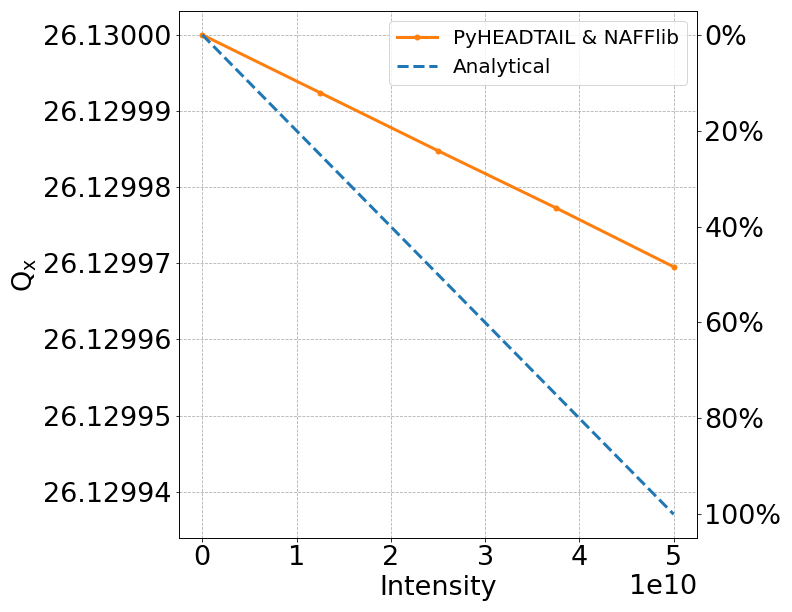
\includegraphics[width=1\textwidth]{images/Ch7/Qx_vs_intensity_complete_impedance_sps_q26model_MD2018_parameters.png}
        %\caption{$y=\sin(2 \pi f t),\ f=50$ Hz}
        %\label{fig:add_label_here}
    \end{subfigure}
    \hfill
    \begin{subfigure}[t]{0.45\textwidth}
        \centering
        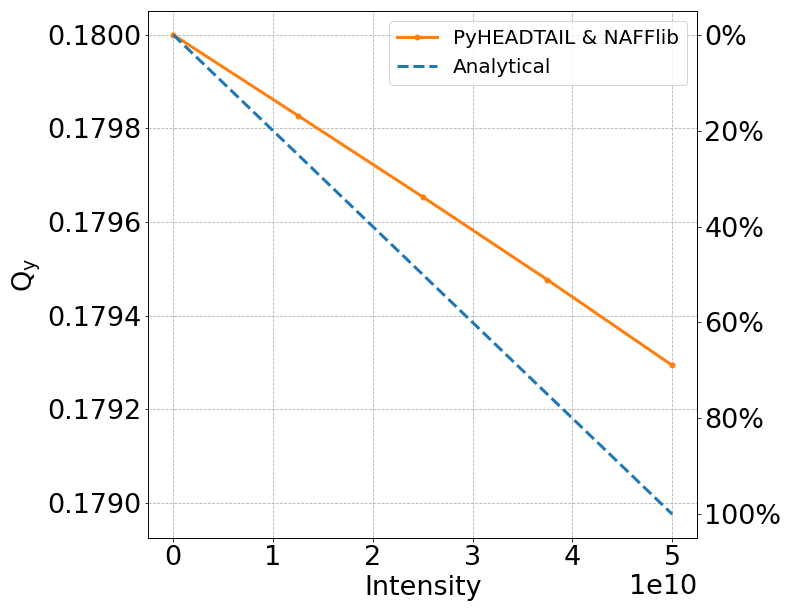
\includegraphics[width=1\textwidth]{images/Ch7/Qy_vs_intensity_complete_impedance_sps_q26model_MD2018_parameters.png}
        %\caption{Discrete Fourier transform}
        %\label{fig:add_label_here}
    \end{subfigure}
    \hfill
     \caption{Horizontal (left) and vertical (right) coherent tunes as a function of intensity in the presence of the beam coupling SPS imepdance obtained using analytical formula (blue dashed line) and PyHEADTAIL tracking simulations (orange line). The impedance model and the wake functions used are available in the public gitlab repository of Ref.~\cite{sps_impedance_model_git}.} % bunch passage
     \label{fig:sps_coherent_DQ_vs_intensity_original_complete_model}
 \end{figure}

 Figure~\ref{fig:sps_coherent_DQ_vs_intensity_original_complete_model} shows that the coherent tune shift from the analytical model does not agree with simulation results. In particular the wakefields implementation in the PyHEADTAIL results just to $\sim 50 \%$ and $\sim 70 \%$ of the total coherent tune shift estimated using the analytical formula of Sacherer with the impedance model. This discrepancy hadn't been observed before as this study has not been conducted for such low intensities (the usual intensity range for this type of study is in the order of $10^{11}$ protons per bunch ~\cite{Beck:2683038}) and short bunches. %p.101
 The analytical predictions from Sacherer formula have been repeatedly successfully benchmarked against beam measurements~\cite{Bartosik:1742183, sps_impedance_measurements_vs_model} which indicates that there is an issue with the model of the wakes or with their implementation in the simualtion. Given the fact that the studies with $\CC$s are quite sensitive on the coherent tune shift with intensity from the coupling impedance (this will be discussed in the following paragraphs of this chapter) it is crucial to identify the reason for the observed discrepancy and resolve it.

 After several studies and discussions with the experts on the topic \footnote{In particular with Carlo Zannini, carlo.zannini@cern.ch.} it was identified that the components of the resistive wall and the step transitions needed to be re-computed to provide higher accuracy at the lower frequencies. The wakes were computed analytically directly in time domain so no FFT is involved (in contrary with the previous discuessed wakefiels). This has the big advantage of removing all the uncertainties introduced by FFT. The details of this work are not discussed here as they are out of the scope of this thesis and they were not performed by the author. The re-computed wake functions along with the rest of the components of the original model can be found in the gihub repository of Ref.~\cite{updated_sps_wakfields_model} and it will be reffered to as the "updated wakefields" model.

 The coherent betatron tune as a function of intensity obtained using PyHEADTAIL and the updated wakefields model is plotted in Fig.~\ref{fig:sps_coherent_DQ_vs_intensity_updated_model} against the analytical predictions from Sacherer formula. In the both transverse planes, the results from the simulations and the theory are in very good agreement ($\leq 5\%$) which is within the uncertainty that one can expect from the model implementation. 

 % pyheadtail_data/final_for_thesis/2018_conditions/study_0_DQ_vs_intensity/
\begin{figure}[!ht]
    \centering
    \begin{subfigure}[t]{0.45\textwidth}
        \centering
        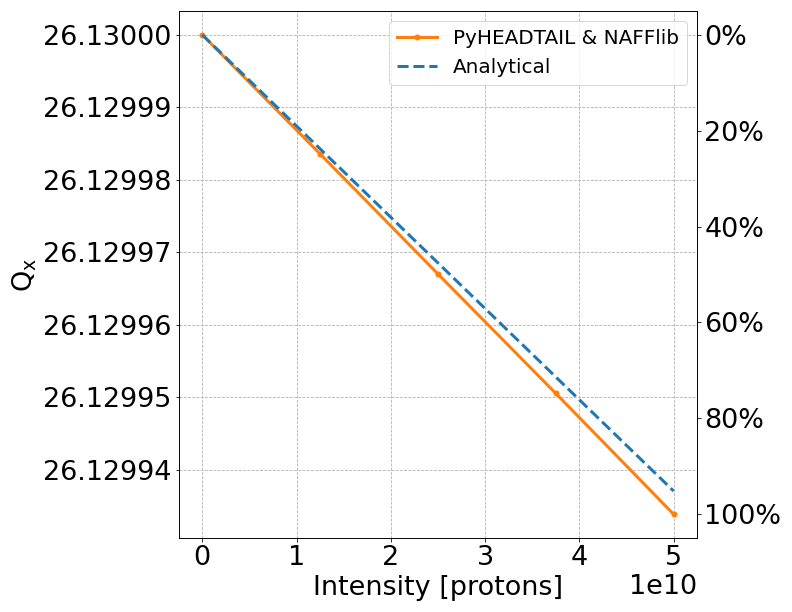
\includegraphics[width=1\textwidth]{images/Ch7/Qx_vs_intensity_complete_impedance_sps_q26model_updated_MD2018_parameters_integer.png}
        %\caption{$y=\sin(2 \pi f t),\ f=50$ Hz}
        %\label{fig:add_label_here}
    \end{subfigure}
    \hfill
    \begin{subfigure}[t]{0.45\textwidth}
        \centering
        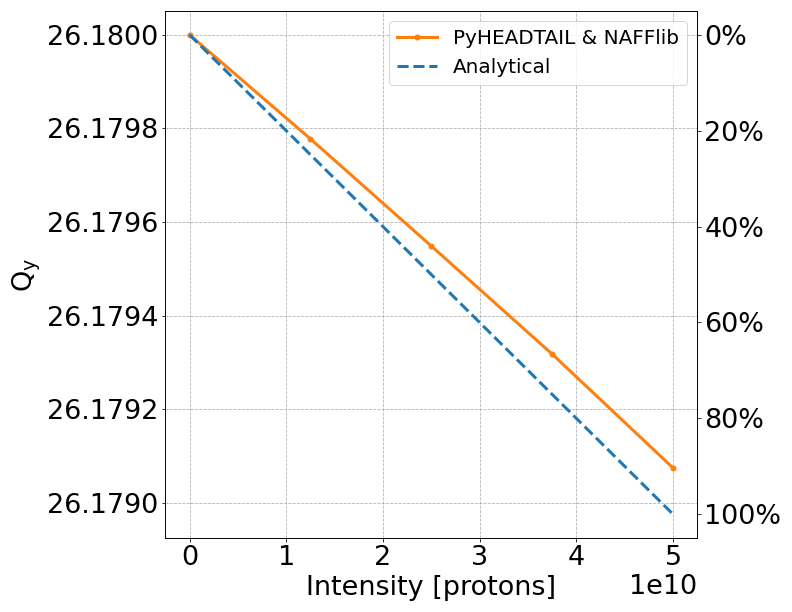
\includegraphics[width=1\textwidth]{images/Ch7/Qy_vs_intensity_complete_impedance_sps_q26model_updated_MD2018_parameters_integer.png}
        %\caption{Discrete Fourier transform}
        %\label{fig:add_label_here}
    \end{subfigure}
    \hfill
     \caption{Horizontal (left) and vertical (right) coherent tunes as a function of intensity in the presence of the beam coupling SPS impedance obtained using analytical formula (blue dashed line) and PyHEADTAIL tracking simulations (orange line). The impedance model and the wake functions ("updated wakefields" model) used are available in the public repositories of Ref.~\cite{sps_impedance_model_git} and Ref.~\cite{updated_sps_wakfields_model} respectively.} % bunch passage
     \label{fig:sps_coherent_DQ_vs_intensity_updated_model}
 \end{figure}

 The above figure demonstrates that the updated wakefields model is reliable and it confirms that its implementation in PyHEADTAIL is correct. Therefore it will be used to study the interplay of the $\CC$ noise induced emittance growth with impedance induced effects. These studies are presented in the following chapter.

 %The above figure confirms the correct implementation of the updated wakefields model in PyHEADTAIL and therefore it will be used to study the interplay of the $\CC$ noise induced emittance growth with impedance induced effects. These studies are presented in the following chapter.

\section{Emittance growth simulations setup}\label{sec:setup_simulations_emit_growth}
The simulations that were performed to investigate the impact of the beam coupling impedance on the $\CC$ RF noise-induced emittance growth were performed following the procedure and using the parameters that are described below. Any change in the choice of parameters, e.g. for some of the parametric studies, will be mentioned in the corresponding paragraph.

The parameters used for setting up the linear transfer map, the longitudinal tracking and the beam initialisation are shown in Table~\ref{tab:pyheadtail_simulation_parameters} and are the ones used in the SPS $\CC$ experiment of 2018. The ring consists of two segments with two interaction points. In the first one, $\CC$ noise-like kicks are applied to the beam particles while in the second one the beam interacts with the wakefields as discussed in the previous section. The updated wakefields model Ref.~\cite{updated_sps_wakfields_model} of the SPS was used.

At the location of the $\CC$ RF noise kick the horizontal and vertical beta functions equal the values at the location of the $\CC2$ which was used in the experiments of 2018. At the location, where the wakefield kicks are applied the transverse beta functions equal the corresponding average beta functions over the SPS machine (see Section~\ref{subsec:pyheadtail}). 

As already discussed in the previous section, the simulations are performed for the Twiss parameter $\alpha_u(s)$ and the dispersion function $D_u(s)$ equal zero. This is a valid assumption for the studies as these parameters have no direct impact on the effects under investigation.

The emittance growth studies were performed for the intensity of $3 \times 10^{10}$ protons per bunch in accordance with the 2018 experiments. The bunch population was represented by $5 \times 10^{5}$ macroparticles and the number of longitudinal slices was 500. The emittance growth was also simulated without including the wakefields. For the latter case, the bunch population was represented by $10^{5}$ particles, and no longitudinal slicing was applied. The studies were performed using an initial Gaussian bunch distribution in the six-dimensional phase space. This is a good approximation for the bunches used in the experimental studies of 2018. 

At the location of the $\CC$ RF noise kick, the angle, $y^\prime$, of each particle within the bunch is updated every turn according to the kicks of Eqs.~\eqref{eq:amplitude_noise_kick} and~\eqref{eq:phase_noise_kick} for amplitude and phase noise kick respectively. The scaling factor, $A$ equals $10^{-8}$ except if it is stated otherwise. This noise level, which corresponds to power spectral density of $1.68 \cdot 10^{-10} \mathrm{rad^2/Hz}$ or $\mathrm{1/Hz}$ for phase and amplitude noise respectively is much stronger than the ones of the actual $\CC$ RF system and was chosen such as it results in a reasonable growth in the simulation time of $10^5$ turns (it corresponds to $\sim$2.5 seconds in the SPS). The emittance growth over the course of the simulation is comparable to that during a coast though. This approach is valid due to the linear growth of emittance with time and the linear scaling with the noise level~\cite{PhysRevSTAB.18.101001}. The parameters used for the implementation of the $\CC$ RF noise kick in the simulations are shown in Table~\ref{tab:CC_pyheadtail_simulation_parameters}.

\begin{table}[!hbt]
	\begin{minipage}{\textwidth}
      \begin{centering}
   \caption{PyHEADTAIL simulation parameters used for the implementation of the CC RF noise kicks for the emittance growth studies. This table is complementary of Table~\ref{tab:CC_pyheadtail_simulation_parameters}.}
	\begin{tabu} to \textwidth {X[c,m] X[0.5c,m] X[0.5c,m] X[0.01c,m]}
		&&& \\[-6mm]
		\toprule \toprule
		\multicolumn{2}{l}{\textbf{Parameter}} &
		\multicolumn{2}{c}{\textbf{Value}} \\
		\bottomrule
      \multicolumn{2}{l}{Horizontal / vertical beta function, $\beta_{x, \mathrm{CC}} / \beta_{y, \mathrm{CC}}$}  & \multicolumn{2}{c}{30.31\,m / 73.82\,m } \\
      \multicolumn{2}{l}{CC frequency, $f_\mathrm{CC}$}  & \multicolumn{2}{c}{400.78\,MHz} \\
      \multicolumn{2}{l}{Scaling factor for amplitude and phase noise, $A$}  & \multicolumn{2}{c}{$10^{-8}$} \\
      \bottomrule
	\end{tabu}
   \label{tab:CC_pyheadtail_simulation_parameters}
   \end{centering}
   \end{minipage}
\end{table}

Last, the emittance growth simulation studies were performed for non-zero linear chromaticity and non-zero detuning with the transverse amplitude. Both effects were introduced as changes in the phase advance of the individual particles according to Eq.~\eqref{eq:change_phase_advance_detunign}. The value of the linear chromaticity, $Q^{\prime}_{x,y}=0.5$ for most of the studies according to the experimental conditions of 2018. Higher-order chromaticities were considered negligible. The values of the detuning coefficients will be given in the following sections.

In the following sections, the emittance growth rates will be expressed in nm/s due to the simulation time scale and will be referred to as the growth of the normalised emittance values to be in agreement with the analysis of the measured data in Chapter~\ref{Ch:2018_analyisis}.

\section{First observations of emittance growth suppression by the impedance}\label{sec:first_obs_suppression}

The first emittance growth simulations were performed for the beam and machine conditions of the 2018 experiments. The parameters are listed in Tables~\ref{tab:pyheadtail_simulation_parameters} and~\ref{tab:CC_pyheadtail_simulation_parameters} and the detailed procedure is described in Section~\ref{sec:setup_simulations_emit_growth}. To give an overview, the study was conducted for a single proton bunch, energy of 270\,GeV, bunch intensity of $3 \times 10^{10}$ protons, rms bunch length $4 \sigma_t = 1.7$\,ns and linear chromaticity of 0.5 in both transverse planes. 

As mentioned in Chapter~\ref{Ch:2018_analyisis} the Landau octupoles were switched off during the 2018 $\CC$ experiment. Nevertheless, a residual non-linearity was present in the machine mainly due to multiple components in the dipole magnets~\cite{Carlà:2664976, Alekou:2640326}. The rms tune spread in the vertical plane from these non-linearities is computed at $\sim$2-3 $\times 10^{-4}$. In order to reproduce this tune spread value in the simualtions, the vertical amplitude detuning coefficient was set at $\alpha_\mathrm{yy}$ = 2000\,1/m. For simplicity, the horizontal and cross-term coefficient were both zero, $\alpha_{xx}=\alpha_{yx}$ = 0.

$\CC$ phase noise was applied as it was the dominant type in the 2018 experiment, with power spectral density of $1.68 \times 10^{-10} \mathrm{rad^2/Hz}$ which corresponds to $A=10^{-8}$ for the scaling factor of Eq.~\eqref{eq:phase_noise_kick}. For this noise power a growth rate of about 25\,nm/s is expected (exciting the first betatron sidebands at $\pm$7.8~\,kHz, see further discussion in Section~\ref{subsec:CC_emit_growth_theoretical_formulas}). 

The geometric emittance value was computed every 100 turns (for computational efficiency) using the statistical definition which can be found in Eq.~\eqref{eq:geometric_emittance_v2}. The emittance growth rate was computed by performing a linear fit to the normalised (using Eq.~\eqref{eq:normalised_emittance}) emittance values over the simualtion turns ($N_\mathrm{turns}=10^5$). Twenty simulation runs were conducted, to reduce the uncertainty of the results. The initial bunch distribution and the sequence of the uncorrelated noise kicks were regenerated randomly for every run. The mean and the standard deviation (including the uncertainty on the slope of the fit) were computed over all the trials.  

The simulations were performed with and without the SPS impedance model to study its impact on the emittance growth induced by $\CC$ RF phase noise. The results are illustrated in Fig.~\ref{fig:MD_2018_impedance_simulations}. The average emittance evolution (over the twenty different runs) in the absence of impedance effects is shown with dark blue color while in the presence of impedance effects with the dark orange color. The shaded areas with light blue and light orange colors show the standard deviation over the twenty runs. The simulated growth without the wakefields is in very good agreement with the theoretically expected growth of $\sim$25\,nm/s (black dashed line). However, once the impedance model is included the phase noise-induced emittance growth blue color is strongly suppressed.

% /eos/user/n/natriant/pyheadtail_data/final_for_thesis/2018_conditions/study_1_MD5_2018_experimental_conditions/job003b_plot_emitGrowth_mutlipleRuns_fillBetween_wakesON_vs_wakesOFF.ipynb
\begin{figure}[!h] 
    \centering         
    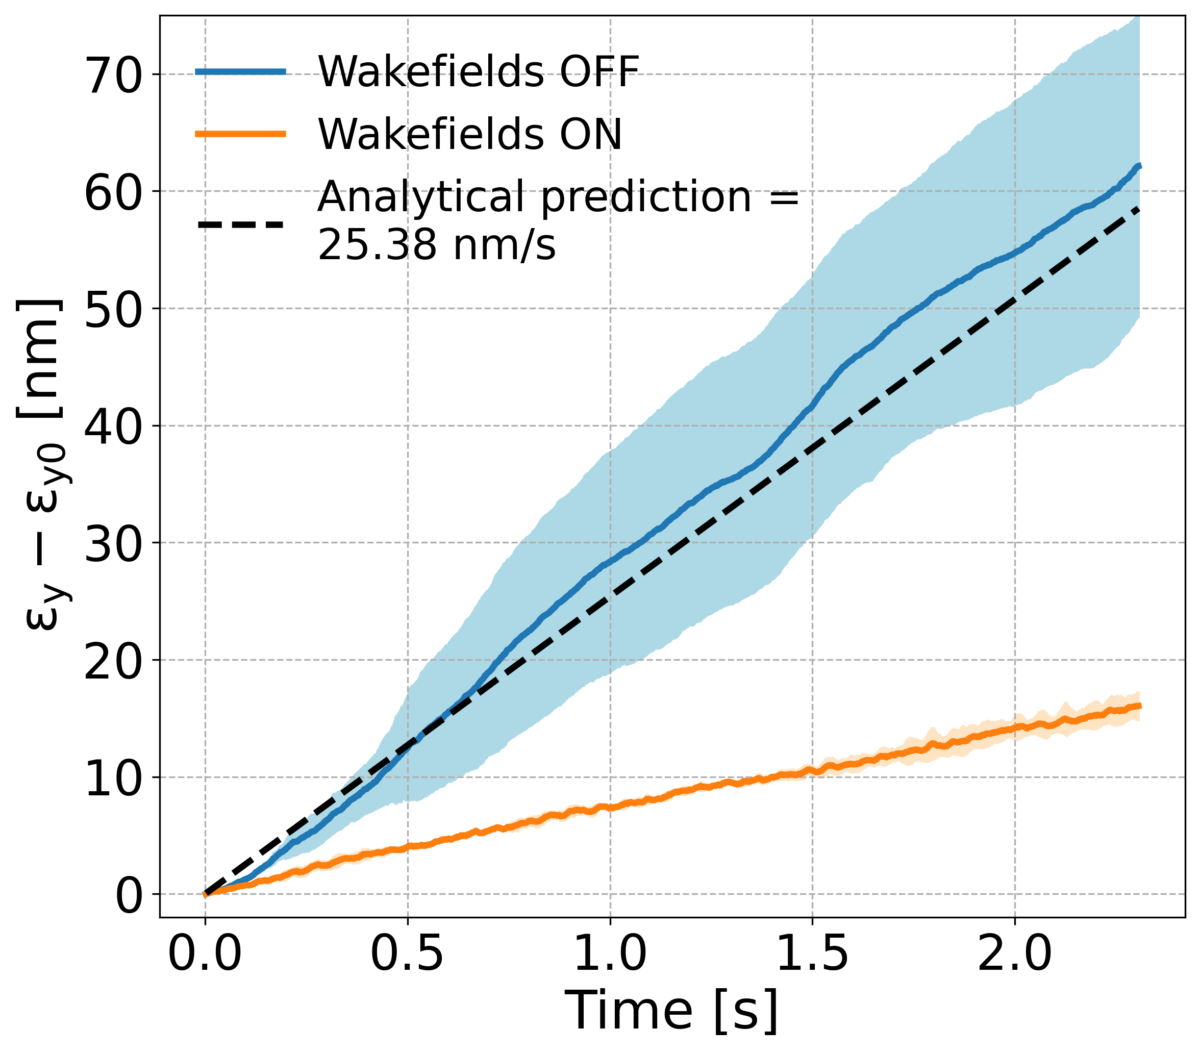
\includegraphics[width=0.85\textwidth]{images/Ch7/sps_270GeV_PN1e-8_400MHz_SPS_NewWakesAllcontributions_appendWakes_y-plane_WakesOFF_QpxQpy5e-1_6D_Nb5e5_intensity3e10_wakesONvsOFF_emittance_evolution.png}
        \caption{Transverse emittance growth driven by CC RF phase noise without (blue) and with (orange) the impedance effects for the beam and machine conditions of the CC tests in SPS during 2018.}
        \label{fig:MD_2018_impedance_simulations}
 \end{figure}

It should be commented, that the big spread in the emittance growth rates over the different simulation runs in the absence of wakefields is a result of the very small tune spread value. The wakefields introduce some additional tune spread, on top of the one from the vertical detuning coefficient, which mitigates the uncertainty of the simulated growth rates

To conclude, PyHEADTAIL simulations showed for the first time that the transverse beam impedance (which is not included in the theory of P.~Baudrenghien and T.~Mastoridis~\cite{PhysRevSTAB.18.101001}) has a significant impact on the emittance growth driven by $\CC$ RF noise. The effect of the suppression of noise-induced emittance growth from the impedance has not been observed before. 
To characterise this effect and to be able to understand the mechanism behind it, a series of exploratory studies were conducted and are discussed in the following section. 


\section{Characterisation of the emittance growth suppression by the impedance}\label{sec:emittance_growth_exploratory_studies}

This section, discusses the results of the exploratory simulation studies which investigate the suppression of the $\CC$ RF noise-induced emittance growth be the transverse beam coupling impedance. The goal is to characterise the effect and understand the mechanism behind it. First, the impact of the imepdance is studied over a range of different amplitude detuning coefficents. Thereafter, in the presence of amplitude noise and in the presence of a noise kick (both in amplitude and phase) from a $\CC$ with the same frequency as the main RF system of the machine (HL-LHC scenario). Then, the effect of the impedance in the presence of a pure dipolar noise kick was simulated followed by a sensitivity study on the impact of the linear chromaticity. Finally, the impact of the dipolar and quadrupolar wakefields was disentangled. 

The simulations were conducted following the same pattern as the case discussed in the previous section. Nevertheless, the main relevant parameters for each case will also be listed in the corresponding section.

\subsection{Sensitivity to amplitude-dependent tune shift}\label{subsec:amplitude_detuning_scan}

As the machine non-linearities were not explicitly characterised during the experiment, the dependence on the octupole-like amplitude dependent tune spread was studied. Instead of using an actual octupolar (non-linear) element which would result to resonance excitation\footnote{In the real SPS machine the Landau octupoles are installed in families of focusing and defocusing in order to avoid the excitation of resonances.}, the amplitude dependent tune shift was introduced as changes to the phase advance of the particles depending on their individual action as discussed in Eq.~\eqref{eq:change_phase_advance_detunign}. More specifically, the dependence on the detuning coefficient in the vertical plane, $\alpha_{yy}$, was studied. In particular $\alpha_{yy}$ ranges from $-$20000 to 20000\,1/m . For the studies presented here and in the following sections of this chapter, the horizontal detuning coefficient and the cross-term were left at zero for simplicity, i.e.~$\alpha_{xx} = \alpha_{xy} = 0$. % for better control over the simulations. This choice is also based on the fact that their value doesn't affect the results.
The sensitivity on the cross-term is discussed in the Chapter~\ref{Ch:experimental_CC_2022}, again for $\alpha_{xy} = 0$ as the horizontal coefficient does not affect the vertical emittance growth since there is no coupling between the two transverse planes.

The simulations were performed with and without the SPS impedance model to study its impact on the emittance growth induced by CC noise. Figure~\ref{fig:MD_2018_impedance_simulations} shows the dependence of the average growth rates (over the twenty different runs) on the amplitude detuning coefficient, $\alpha_{yy}$. The error bars indicate the standard deviation between those twenty runs. The secondary horizontal axis shows the resulting rms tune spread computed using Eq.~\eqref{eq:rms_amplitute_detuning_3}. Incoherent tune shift from other sources, than the detuning with transverse amplitude are not included. In particular, the effect of chromaticity is not taken into account in the computation of the tune spread as it varies periodically with the synchrotron period \textcolor{red}{(does it cancel out?)} and the incoherent tune shift from the impedance is considered negligible. 

\begin{figure}[!h] % at the directory of ipac22
    \centering         
    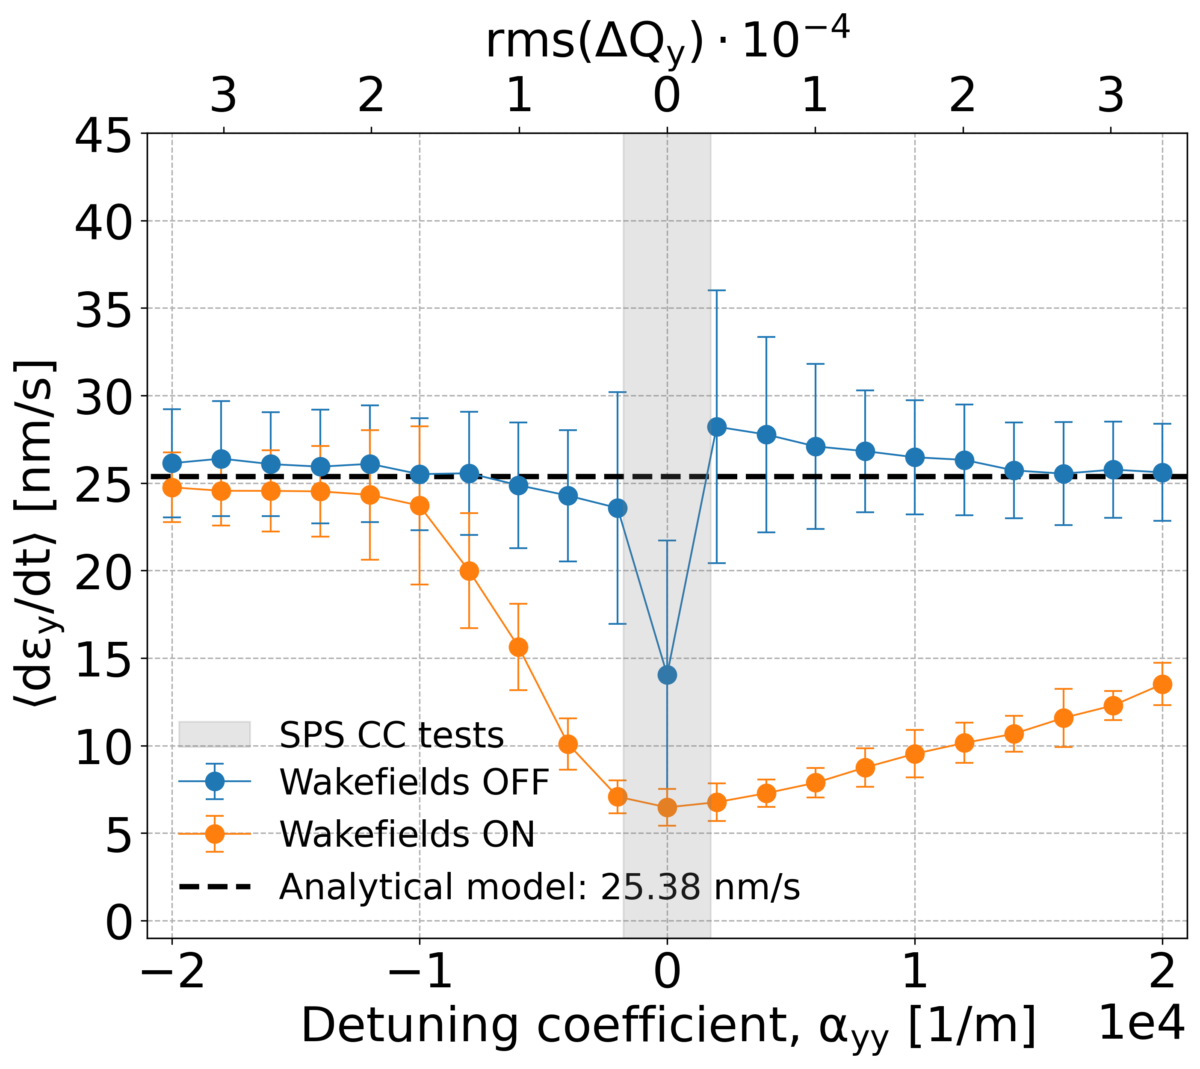
\includegraphics[width=0.85\textwidth]{images/Ch7/deyRates_final_2018_PN_sps_270GeV_PN1e-8_400MHz_y-plane_QpxQpy5e-1_6D_Nb5e5_intensity3e10_ayyScan_wakesON_vs_OFF_vs_TuneSpreadvsExpectedSPS.png}
        \caption{Transverse emittance growth driven by CC RF phase noise without (blue) and with (orange) the impedance effects as a function of tune spread.}
        \label{fig:MD_2018_impedance_simulations_amplitude_detuning}
 \end{figure}

It can be seen that when the wakefield kicks are not applied on the beam the emittance growth rate agrees very well with the value predicted by Eq.~\eqref{eq:dey_pn} and (within the reproducibility of the simulation) is independent of the tune spread value. It should be noted that the theoretical model is not valid for zero tune spread, and that the observed emittance growth rate for $\alpha_{yy} = 0$ is a result of the geometric distortion of the beam caused by the $\CC$ kick.

Figure~\ref{fig:MD_2018_impedance_simulations} also shows a clear suppression of the transverse emittance growth when the wakefield kicks are included. The suppression depends on the tune spread and is asymmetric for positive and negative values of the detuning coefficient. Over a realistic range of tune spread values (estimated with MAD-X~\cite{madx} including the non-linearities of SPS~\cite{Carlà:2664976, Alekou:2640326} and $Q^\prime_{x,y}$ = 0.5, and shown by the grey shaded area in Fig.~\ref{fig:MD_2018_impedance_simulations}) the suppression reaches up to a factor 4-5. This suppression is very close to that observed in the experiments and suggests that the impedance effects might explain the discrepancy between the measured and theoretically estimated emittance growth rates.


\subsection{Amplitude noise}\label{subsec:amplitude_noise}
The simulations discussed here were performed with and without the SPS imepdance model in the presence of $\CC$ RF amplitude noise, with power spectral density of $1.68 \times 10^{-10}$ 1/Hz which corresponds to $A=10^{-8}$ for the scaling factor in Eq.~\eqref{eq:amplitude_noise_kick}. The amplitude of the amplitude noise kicks equals the one of the phase noise kicks used in the previous section. The results are shown in Fig.~\ref{fig:study_1_2018_paramters_AN}.

\begin{figure}[!h] % at the directory of ipac22
    \centering         
    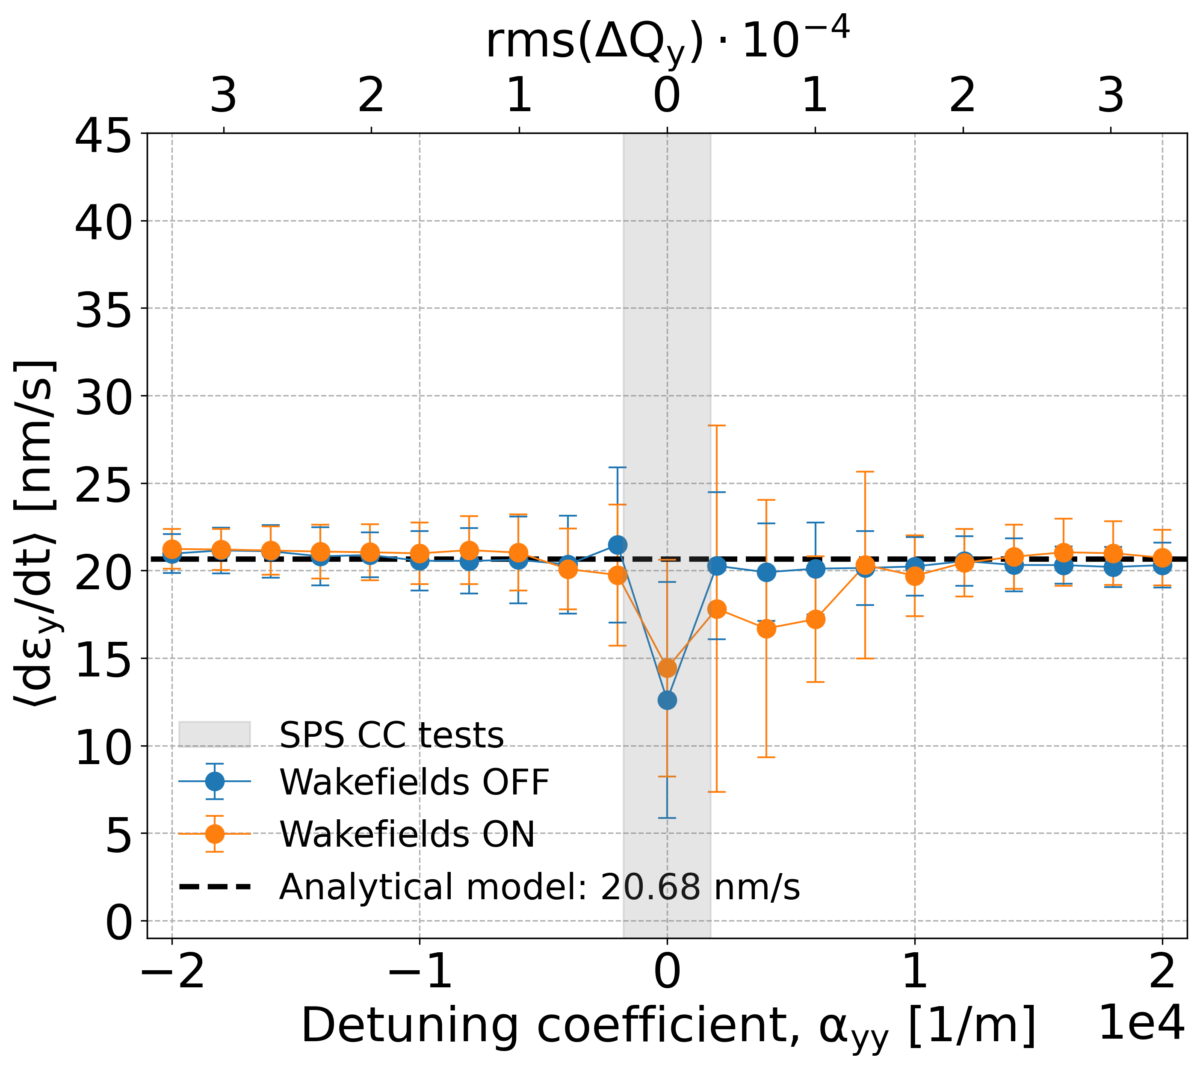
\includegraphics[width=0.85\textwidth]{images/Ch7/deyRates_final_2018_AN_sps_270GeV_AN1e-8_400MHz_y-plane_QpxQpy5e-1_6D_Nb5e5_intensity3e10_ayyScan_wakesON_vs_OFF_vs_TuneSpreadvsExpectedSPS.png}
        \caption{Transverse emittance growth driven by CC RF amplitude noise without (blue) and with (orange) the impedance effects as a function of tune spread.}
        \label{fig:study_1_2018_paramters_AN}
 \end{figure}

 It can be seen that the emittance growth rate agrees very well with the value predicted by Eq.~\eqref{eq:dey_an} and (within the reproducibility of the simulation) is independent of the tune spread value both when the wakefields are included and when they are not. In other words, the simulations demonstrate that the emittance growth driven by $\CC$ RF amplitude noise (which is associated with the headtail mode 1) is not suppressed by impedance induced effects. As the phase noise kick is similar to a dipolar noise kick (headtail mode 0) but with a high order distortion it seems that the suppression form the impedance is related to the dipole motion.


 \subsection{CC RF noise at 200\,MHz}\label{subsec:fcc_200MHz}
Now, the study was repeated for $\CC$ RF noise kick at 200\,MHz, i.e. $\CCfrequency=200$\,MHz, which equals the frequency of the main accelerating RF system of the SPS (see Table~\ref{tab:machine_beam_param_2018}). The main reason for this study is that in that case in the presence of phase (amplitude) noise the headtail mode 0 (1) is more dominant than in the case of RF noise at 400\,MHz. Additionally, this is also similar to the HL-LHC scenario where the main RF system and the $\CC$s will operate at the same frequency ($f_\mathrm{C, }=f_\mathrm{RF, HL-LHC}$=400\,MHz).

The simulations were performed with and without the SPS impedance model in the presence of both amplitude and phase noise with power spectral density of $1.21 \times 10^{-10} \mathrm{rad^2/Hz}$ (A=$10^{-8}\sqrt{0.72}$) and $3.06 \times 10^{-10} \mathrm{1/Hz}$ (A=$10^{-8}\sqrt{1.82}$) respectively. The noise strength was scaled such as it results in $\sim$ 25 nm/s to be comparable with the initial studies presented in Section~\ref{sec:first_obs_suppression}.

The PyHEADTAIL simulation results are summarised in Fig.~\ref{fig:CC_200MHz_amplitude_phase_noise}. The first plot (left) displays the amplitude detuning dependent emittance growth in the presence of amplitude noise while the second plot (right) in the presence of phase noise. 

% amplitude noise: pyheadtail_data/final_for_thesis/2018_conditions/study_4_amplitude_noise_200MHz
% phase noise: pyheadtail_data/final_for_thesis/2018_conditions/study_3_phase_noise_200MHz
\begin{figure}[!ht]
    \centering
    \begin{subfigure}[t]{0.45\textwidth}
        \centering
        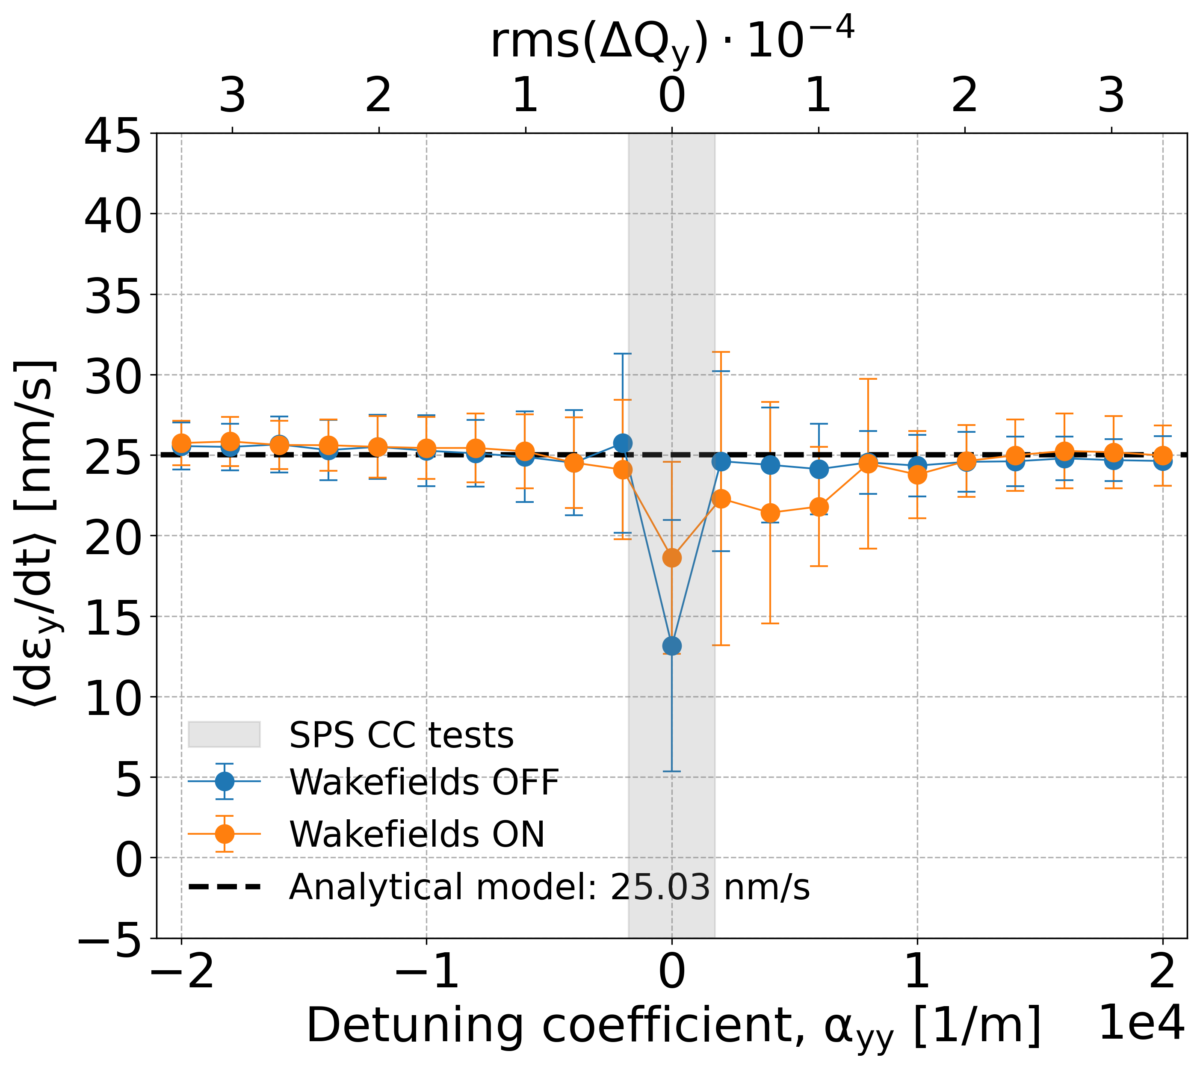
\includegraphics[width=1\textwidth]{images/Ch7/deyRates_final_2018_AN_sps_270GeV_PN1e-8_200MHz_y-plane_QpxQpy5e-1_6D_Nb5e5_intensity3e10_ayyScan_wakesON_vs_OFF_vs_TuneSpreadvsExpectedSPS_200MHz.png}
        \caption{Amplitude noise}
        %\label{fig:add_label_here}
    \end{subfigure}
    \hfill
    \begin{subfigure}[t]{0.45\textwidth}
        \centering
        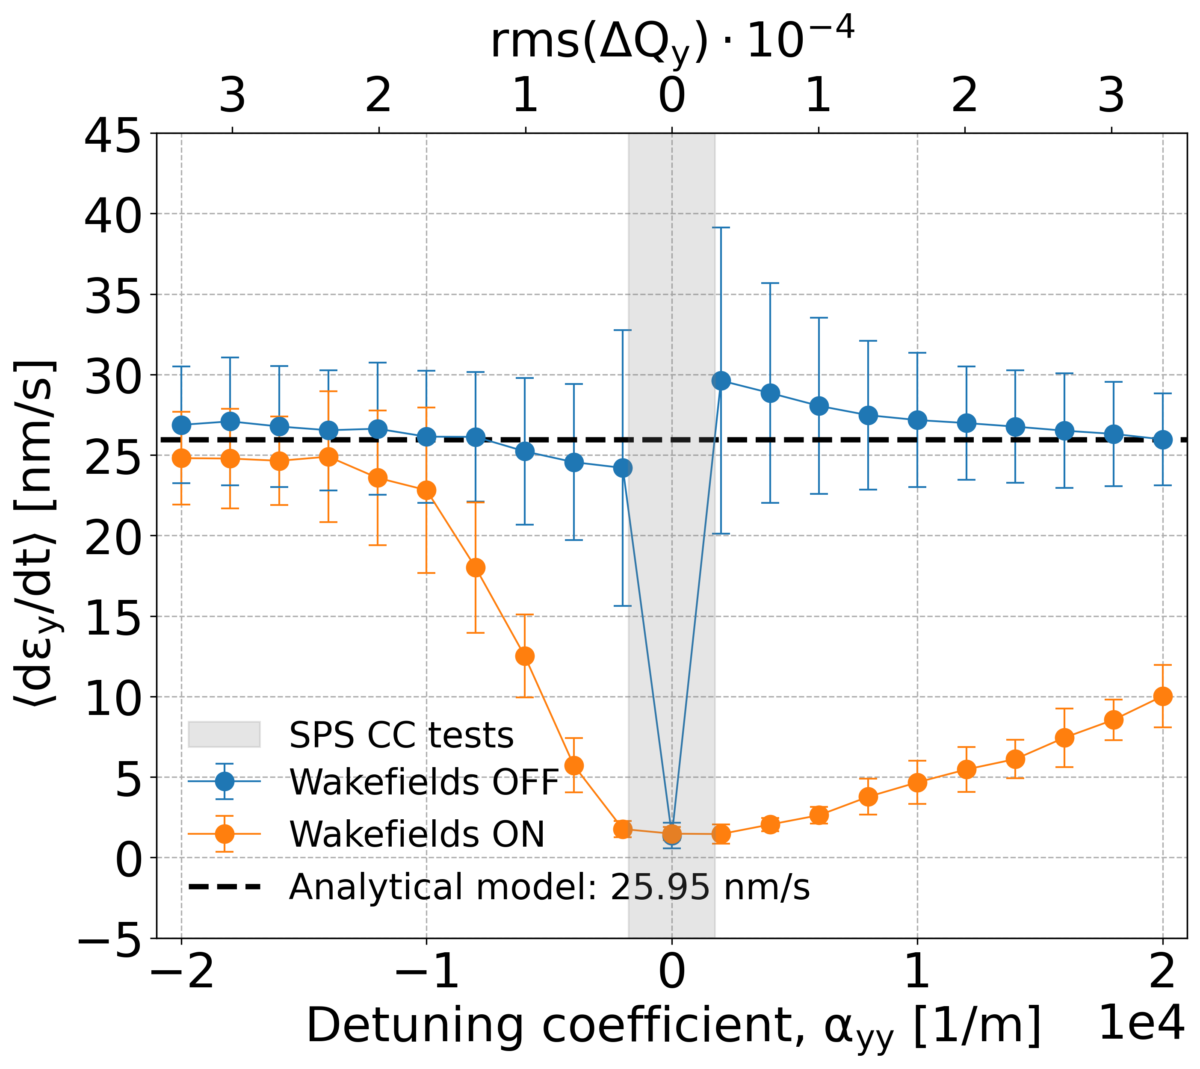
\includegraphics[width=1\textwidth]{images/Ch7/deyRates_final_2018_PN_sps_270GeV_PN1e-8_200MHz_y-plane_QpxQpy5e-1_6D_Nb5e5_intensity3e10_ayyScan_wakesON_vs_OFF_vs_TuneSpreadvsExpectedSPS_200MHz.png}
        \caption{Phase noise}
        %\label{fig:add_label_here}
    \end{subfigure}
    \hfill
     \caption{Transverse emittance growth driven by CC RF noise at $\CCfrequency=$200\,MHz without (blue) and with (orange) the impedance effects as a function of tune spread.} % bunch passage
     \label{fig:CC_200MHz_amplitude_phase_noise}
 \end{figure}

 Comparing Fig.~\ref{fig:CC_200MHz_amplitude_phase_noise} (left) and Fig.~\ref{fig:study_1_2018_paramters_AN} it becomes evident that the behavior of the amplitude noise induced emittance growth is consistent for noise at 200 and 400\,MHz (both with and without wakefields). In both cases there is no amplitude detuning dependent suppression of the emittance growth while the obtained growth rates agree very well with the theoretical predictions from Eq.~\eqref{eq:dey_an}.
 
 Comparing Fig.~\ref{fig:CC_200MHz_amplitude_phase_noise} (right) and Fig.~\ref{fig:MD_2018_impedance_simulations} it can be seen that emittance growth driven by $\CC$ phase noise in the absence of wakefield kicks (blue) is in excellent agreement for noise at 200 and 400\,MHz except for the case with zero amplitude detuning, $\alpha_\mathrm{yy}=0$. It is already discussed, that for $\CCfrequency$=400\,MHz the observed emittance growth of $\sim 15$\,nm/s is a result of the geometric distortion of the beam caused by the $\CC$ kick. This geometric distortion is minimised when the frequency of the $\CC$ kick equals the one of the main RF system hence the almost zero emittance growth observed for the phase noise at 200\,MHz. 

 Repeating the last comparison but in the presence of wakefield kicks (orange) it can be seen that emittance growth driven by $\CC$ phase noise is in good agreement with the results for noise at 200 and 400\,MHz. The suppression of the emittance growth, which depends on the amplitude detuning, is observed in both cases. However, in the case of phase noise at 200\,MHz the suppression factor reaches up to a factor of 10 instead of just 4-5 in the case of noise at 400\,MHz. The enhanced effect of suppression in the case where the $\CC$ has the same frequency with the main RF system of the machine and thus the headtail mode 0 is dominant provides an additional argument that the emittance growth suppression from the beam coupling impedance is associated to that mode. To this end, as a next step the emittance growth induced by a pure dipolar noise is studied.


 %Comparing Fig.~\ref{fig:CC_200MHz_amplitude_phase_noise} (right) and Fig.~\ref{fig:MD_2018_impedance_simulations} it can be seen that emittance growth driven by $\CC$ phase noise in the presence of wakefield kicks (orange) is in good agreement for noise at 200 and 400\,MHz. 


\subsection{Pure dipolar noise}\label{subsec:dipole_noise}
To validate that the effect of the suppression of the noise-driven emittance growth from the beam coupling impedance is associated with the dipolar motion (headtail mode 0), the same simulations as in the previous part were conducted but instead of the longitudinally dependent noise kicks a pure dipolar noise kick was applied on the beam. The dipolar noise kick was modeled by the transformation of Eq.~\eqref{eq:external_noise_kicks} for $A=10^{-8} \sqrt{2}$ which corresponds to a power spectral density of 3.36\,$\mathrm{rad^2/Hz}$. The noise strength was scaled such as it results in $\sim$ 25 nm/s to be comparable with the initial studies presented in Section~\ref{sec:first_obs_suppression}.

Figure~\ref{fig:study_5_dipole_noise} shows the noise-induced vertical emittance growth as a function of amplitude-dependent tune spread with and without the presence of wakefield kicks. One can see that in the absence of wakefields (blue) the behavior of the dependence of the growth rates on the amplitude detuning matches the one obtained from $\CC$ RF phase noise kicks (see Figs.~\ref{fig:study_1_2018_paramters_AN} and~\ref{fig:CC_200MHz_amplitude_phase_noise} (right)). However, now, due to the absence of any geometric distortion for $\alpha_\mathrm{yy}=0$ there is zero emittance growth as one would expect from the fact that the models that predict the emittance growth are not valid for zero tune spread.

In the presence of wakefield kicks (orange) a very strong suppression of the emittance growth is suppressed which reaches up to a factor of 10 for the small values of amplitude detuning (within the gray area which indicates the tune spread present in the SPS during the 2018 $\CC$ experiments). The fact that the suppression of the emittance growth intensifies in the presence of dipolar noise, is a way to infer the association of the phenomenon with the headtail mode 0.

\begin{figure}[!h] % cernbox/=/pyheadtail_data/final_for_thesis/2018_conditions/study_5_dipole_nois
    \centering         
    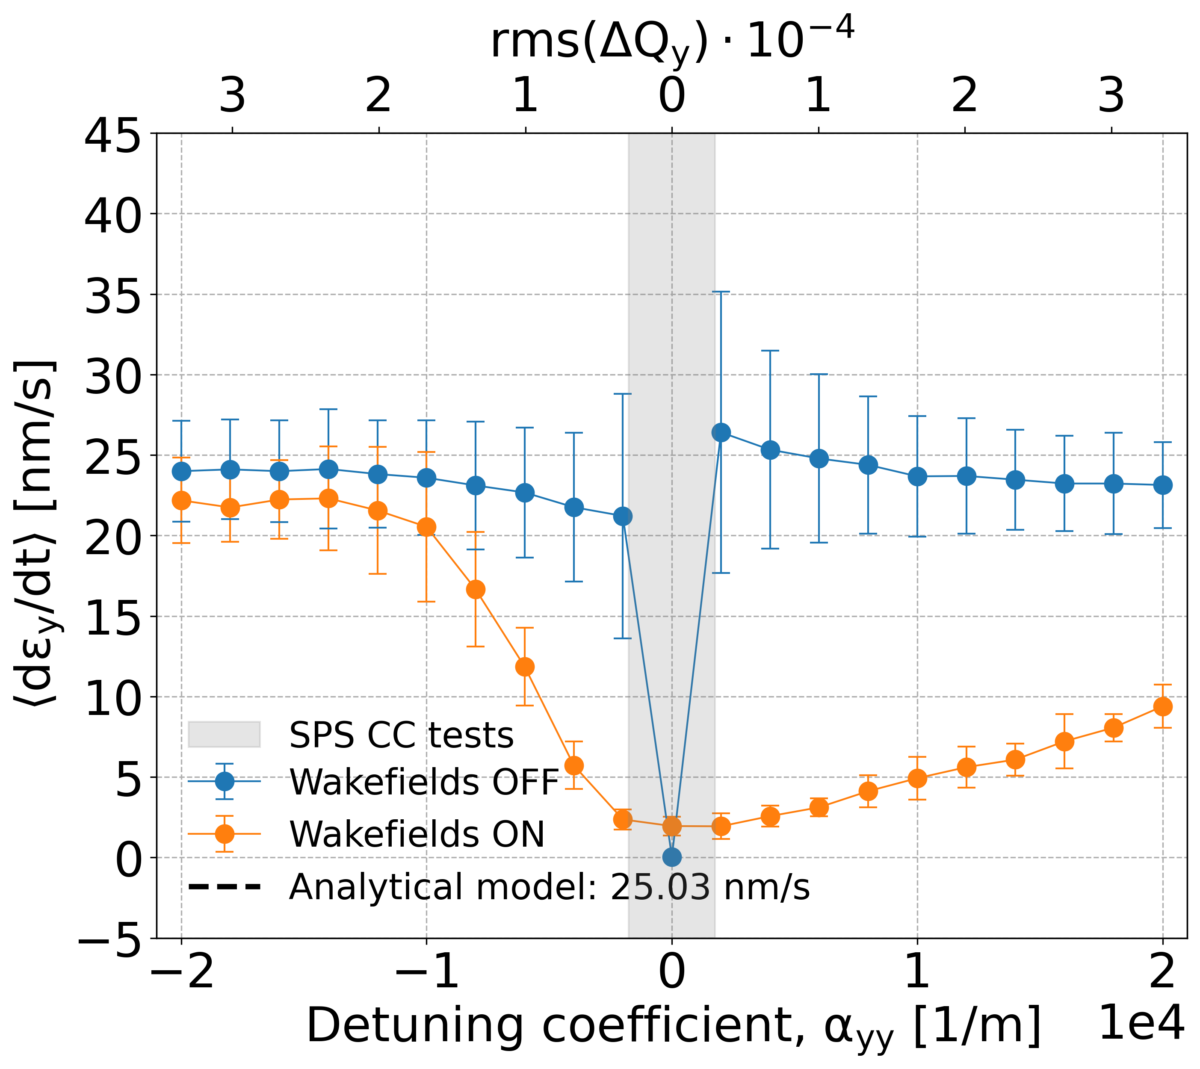
\includegraphics[width=0.7\textwidth]{images/Ch7/deyRates_final_2018_PN_sps_270GeV_DipoleNoiseSQRT1e-8_y-plane_QpxQpy5e-1_6D_Nb5e5_intensity3e10_ayyScan_wakesON_vs_OFF_vs_TuneSpreadvsExpectedSPS.png}
        \caption{Transverse emittance growth driven by a pure dipolar noise kick without (blue) and with (orange) the impedance effects as a function of tune spread.}
        \label{fig:study_5_dipole_noise}
 \end{figure}

\subsection{Sensitivity to linear chromaticity}\label{subsec:chroma_scan}
The PyHEADTAIL simulations discussed up to now, cover the case for linear chromaticity $Q^\prime_{x,y}=0.5$ which is believed to be the case for the emittance growth measurements in SPS in 2018. To understand the effect of the linear chromaticity on the suppression of the noise-induced emittance growth from the SPS impedance the same simulation as in Section~\ref{sec:first_obs_suppression} were repeated over a range of different chromaticities. In particular, five different values were studied: $Q^\prime_{x,y}=0.0, 0.5, 1.0, 2.5, 5.0$. It can be seen, that the study is limited to small positive chromaticity values following past experimental chromaticity scans for emittance growth studies,  $Q^\prime_{x,y}< 10.0$~\cite{Antoniou:2649815, Calaga:1451286}. An additional reason for not extending the study to the negative chromaticity values is that they would lead to beam instabilities.
% Note 1: The expereimental scan of the linear chromaticity scan from 0 to 7 (rama's paper), ipac2012.
% Note 2: if needed you can prove that the beam is unstable with the formula of Sacherer.

As already mentioned, the simulations for this subsection were performed using the setup and the parameters of Section~\ref{sec:first_obs_suppression}. This means, that the study took place in the presence of $\CC$ RF phase noise kicks at 400\,MHz, with and without including the SPS imepdance model. The results of the scan in $Q^\prime_{x,y}$ are displayed in Fig.~\ref{fig:study_6_chroma_scan} where each subfigure pictures the results for each chromaticity value independently, increasing in value from top left to bottom right. 
\begin{figure}[htp]
    \centering
    \begin{subfigure}{.45\textwidth}
        \centering
        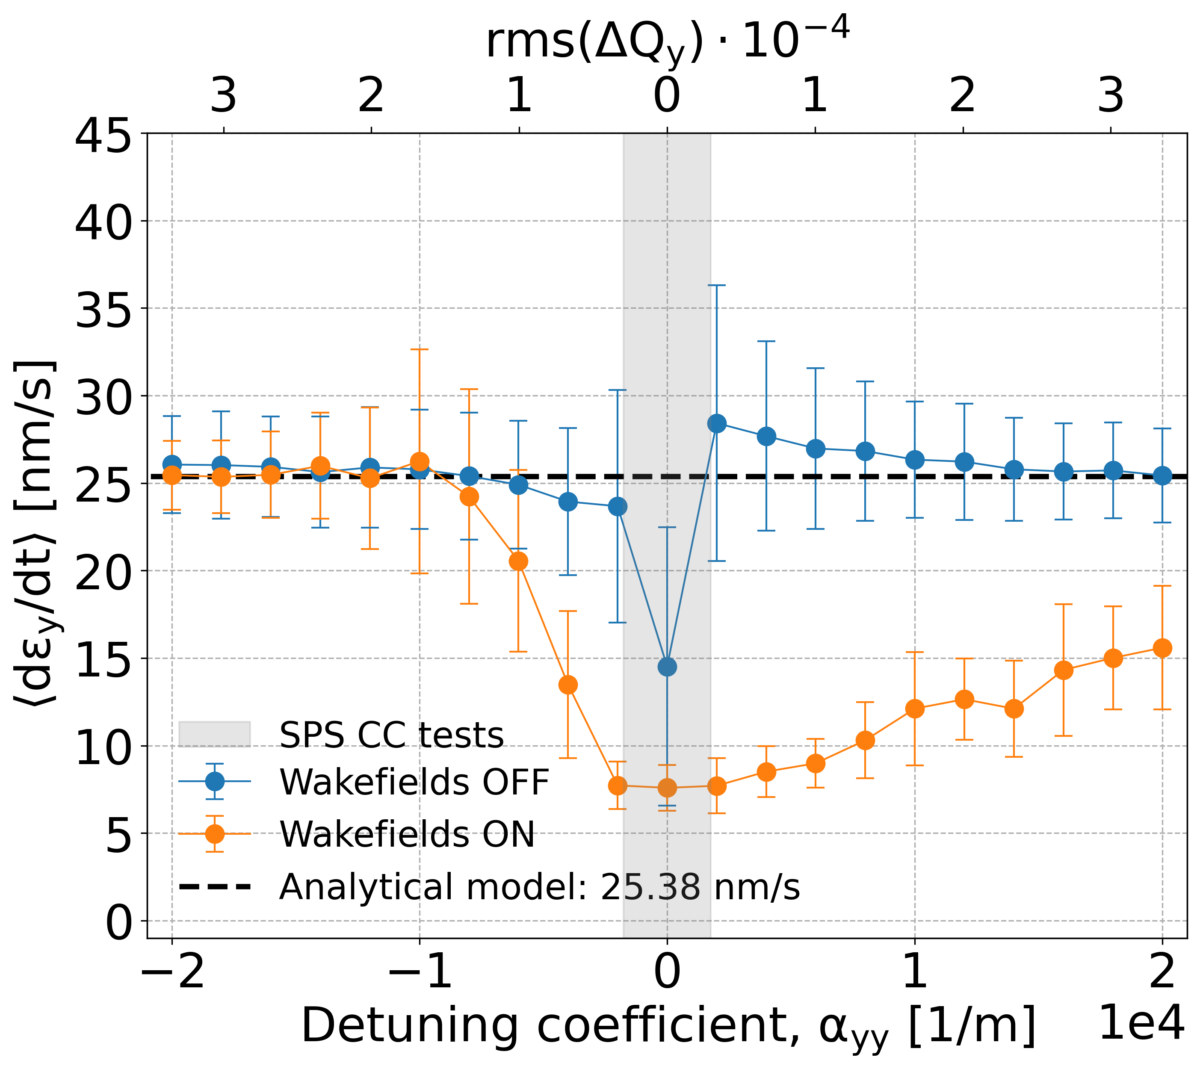
\includegraphics[width=.95\linewidth]{images/Ch7/Qpx0.png}  
        \caption{$Q^\prime_{x,y}$=0.0}
        \label{fig:study_6_chroma_scan_Qpxy0}
    \end{subfigure}
    \begin{subfigure}{.45\textwidth}
        \centering
        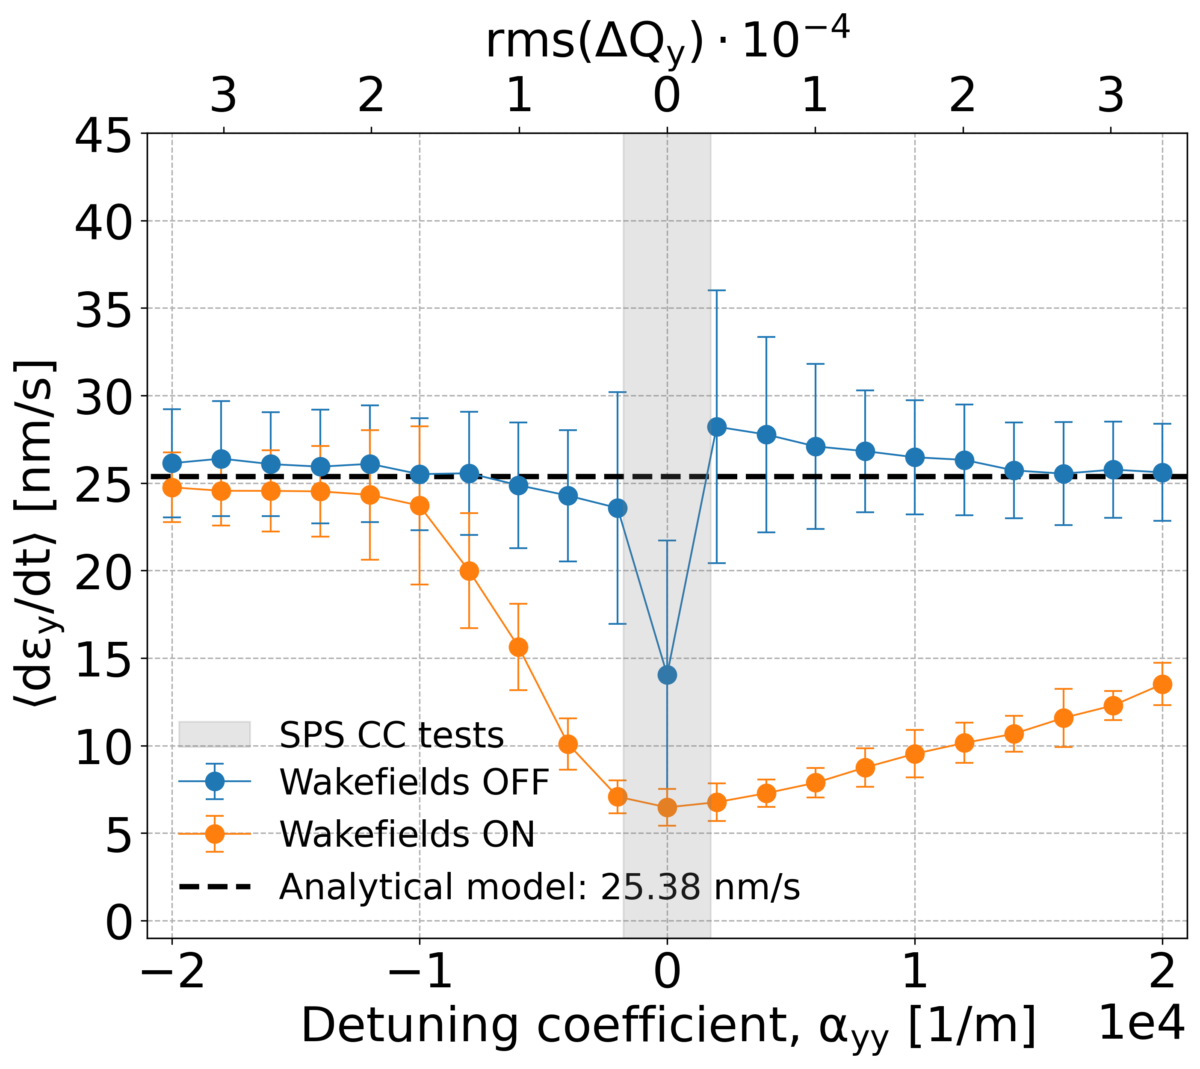
\includegraphics[width=.95\linewidth]{images/Ch7/deyRates_final_2018_PN_sps_270GeV_PN1e-8_400MHz_y-plane_QpxQpy5e-1_6D_Nb5e5_intensity3e10_ayyScan_wakesON_vs_OFF_vs_TuneSpreadvsExpectedSPS.png}
        \caption{$Q^\prime_{x,y}$=0.5}
        \label{fig:study_6_chroma_scan_Qpxy5e-1}
    \end{subfigure}
    \begin{subfigure}{.45\textwidth}
        \centering
        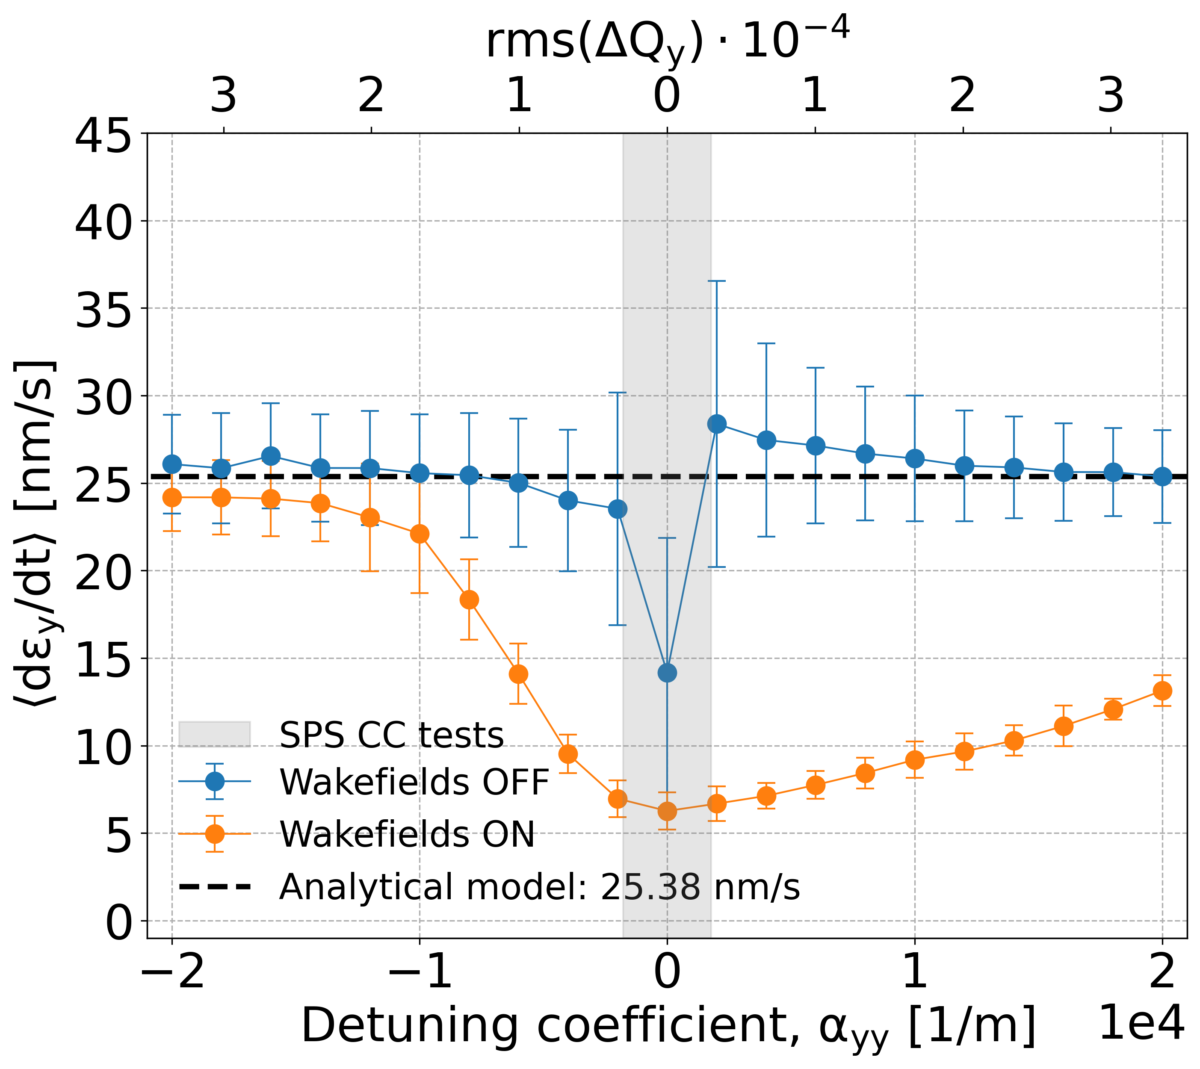
\includegraphics[width=.95\linewidth]{images/Ch7/Qpx1.png}  
        \caption{$Q^\prime_{x,y}$=1.0}
        \label{fig:study_6_chroma_scan_Qpxy1}
    \end{subfigure}
    \begin{subfigure}{.45\textwidth}
        \centering
        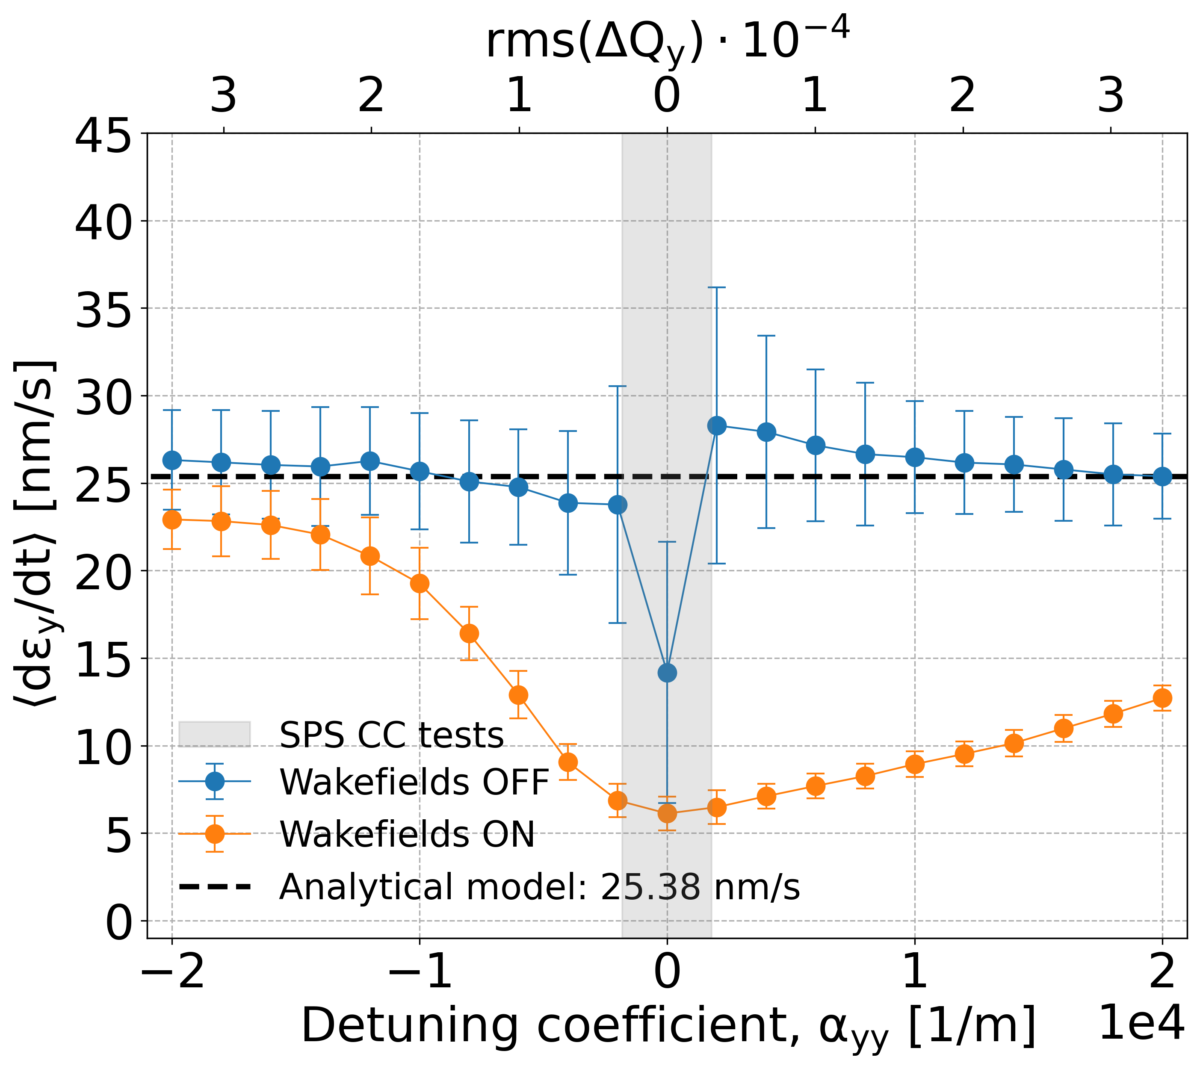
\includegraphics[width=.95\linewidth]{images/Ch7/Qpx25e-1.png}  
        \caption{$Q^\prime_{x,y}$=2.5}
        \label{fig:study_6_chroma_scan_Qpxy25e-1}
    \end{subfigure}
    \begin{subfigure}{.45\textwidth}
        \centering
        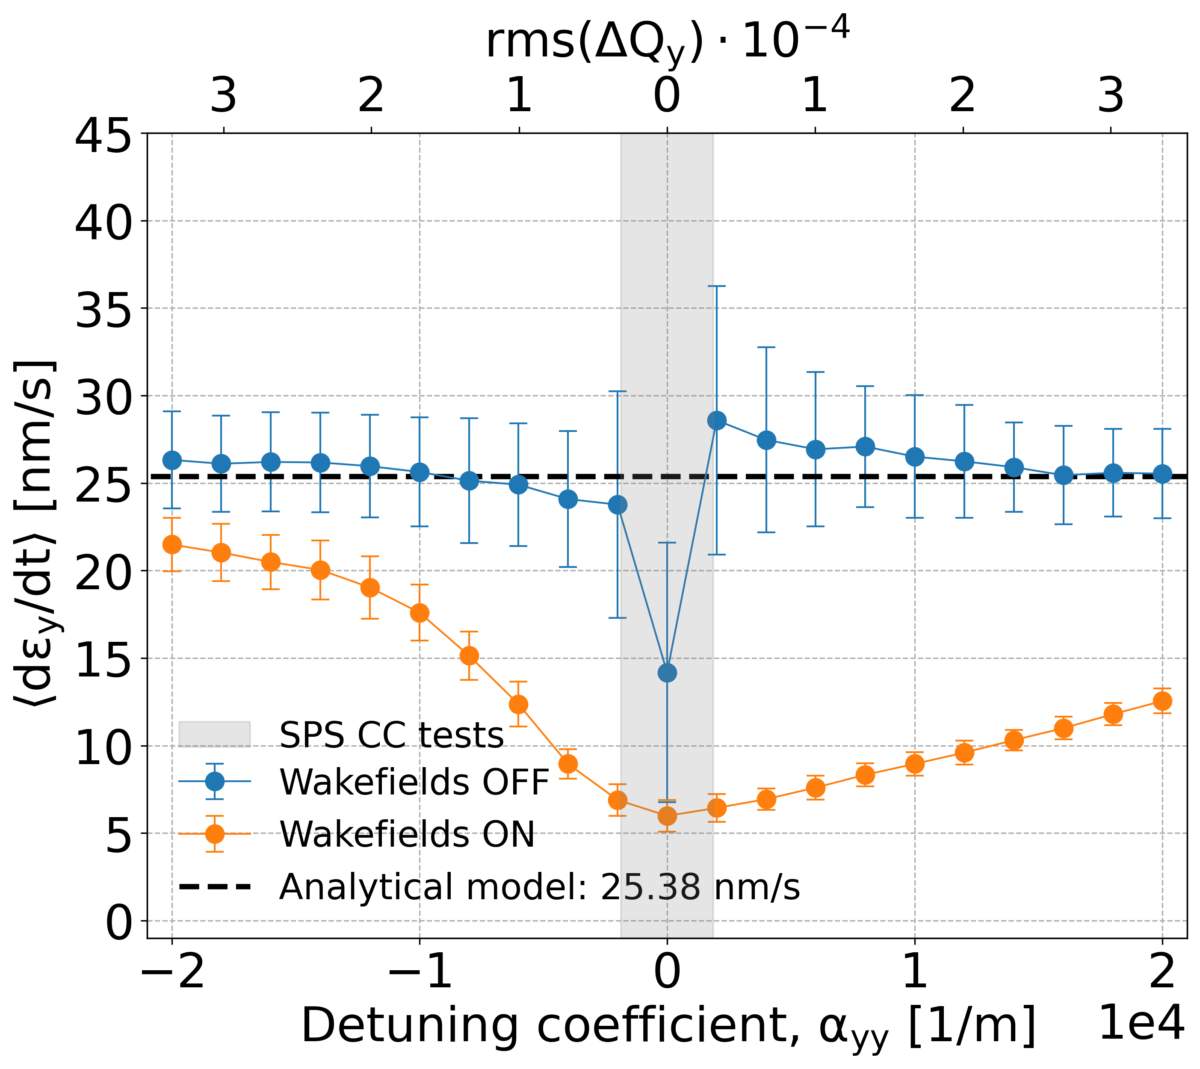
\includegraphics[width=.95\linewidth]{images/Ch7/Qpx5.png}  
        \caption{$Q^\prime_{x,y}$=5.0}
        \label{fig:study_6_chroma_scan_Qpxy5}
    \end{subfigure}
    \caption{Transverse emittance growth driven by CC RF phase noise at 400\,MHz without (blue) and with (orange) the impedance effects as a function of tune spread is shown for five different values of linear chromaticity increasing from top left to bottom right.}
    \label{fig:study_6_chroma_scan}
\end{figure}

In the absence of impedance effects (blue), the $\CC$ RF noise-induced emittance growth rates appear independent of both the amplitude detuning coefficient and the value of linear chromaticity. This is in agreement, with the predictions of the theory developed by T.~Mastoridis and P.~Baudrenghien~\cite{PhysRevSTAB.18.101001} for the white noise spectrum.

In the presence of impedance effects (orange), the suppression of the emittance growth is observed for all the studied values of linear chromaticity. An examination of the results shows that the impact of the linear chromaticity on the maximum suppression, which is observed for $\alpha_\mathrm{yy}=0$, is negligible. Yet, the simulated emittance growth rates exhibit a slightly different dependence on the vertical detuning coefficient, $\alpha_\mathrm{yy}$, for each of the five chromaticity values. This difference appears mainly for the negative values of $\alpha_\mathrm{yy}$. In particular, it appears that for increasing linear chromaticity, the provided tune spread from amplitude detuning is becoming less sufficient for recovering the emittance growth rates expected from the theory of T.~Mastoridis and P.~Baudrenghien~\cite{PhysRevSTAB.18.101001}. Nevertheless, for the regime of the realistic SPS tune spread (grey stripe) the dependence of the suppression factor on the chromaticity appears negligible. This confirms, that the fact that there are no exact measurements available from the SPS $\CC$ tests of 2018, is not a significant issue. 

%Last, it is observed that for increasing chromaticity value the dependence of the growth rates on the detuning coefficient appears less wiggly. Maybe is because of less tune spread, thus larger undertainty? On the other hand the dependence on the linear chromaticity shouldn't play a role.

This small dependence of the shape of the suppression curve (shaped from the emittance growth rates for different values of detuning coefficient) on the linear chromaticity is not surprising as the damping or growth time of headtail mode 0, depends on it (see Eq.~\eqref{eq:imaginary_tune_mode_l}). Nevertheless, overall, it can be concluded that there is no significant sensitivity of the suppression induced by the beam coupling impedance to the linear chromaticity. 

\subsection{Disentangling quadrupolar and dipolar impedance contributions}\label{subsec:quad_vs_dipole}
The simulation described in Section~\ref{sec:first_obs_suppression} is repeated one more time here, with the goal being to disentangle the quadrupolar (detuning) and dipolar (driving) terms of the wakefields to see which one results to the emittance growth suppression. This is easily achievable since in the SPS impedance model the quadrupolar and dipolar terms are provided separately (see Section~\ref{sec:sps_impedance_model}) and thus one can easily select which one to include or exclude from the PyHEADTAIL simulation. The linear chromaticity for this study was corrected to $Q^\prime_{x,y}$=0.5 units.

The results are summarised in Fig.~\ref{fig:study_7_dipole_vs_quadrupole}. The upper plots illustrate the individual effect of the dipolar (left) and quadrupolar (right) terms of the SPS wakefields on the noise-induced emittance growth while the bottom plot shows the combined effect of the two terms. For each study case, the simulation results without including the impedance effects are also shown (blue) for reference. As always, the obtained growth rates appear independent of the vertical detuning coefficient and are in very good agreement (within the errorbars) with the theoretical predictions of the model of T.~Mastoridis and P.~Baudrenghien~\cite{PhysRevSTAB.18.101001} which doesn't take into account impedance effects.

\begin{figure}[htp]
    \centering
    \begin{subfigure}{.45\textwidth}
        \centering
        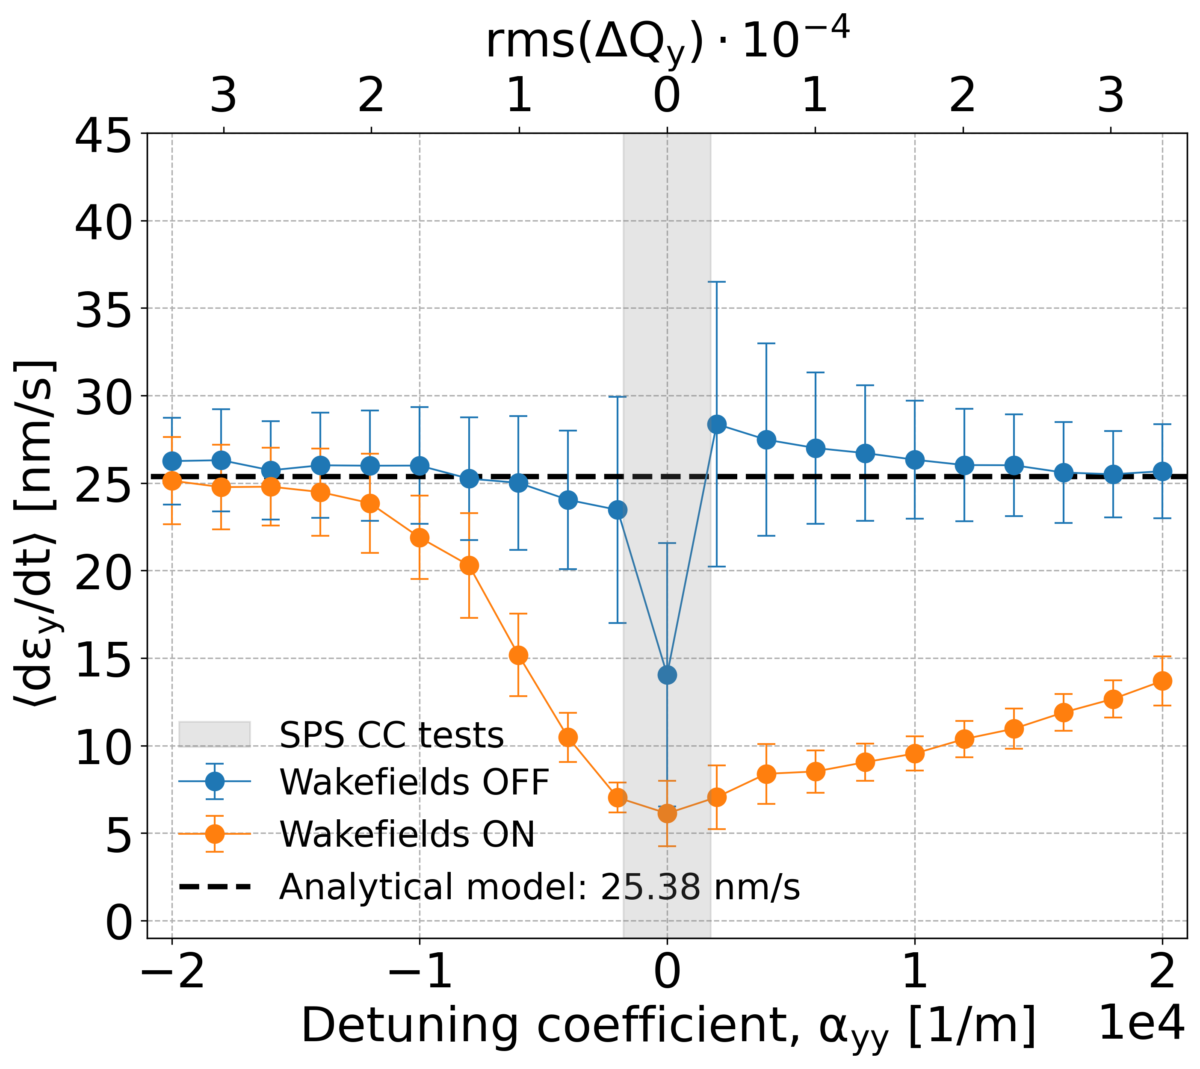
\includegraphics[width=.95\linewidth]{images/Ch7/dipolar_impedance.png}  
        \caption{Only dipolar (driving) impedance contribution.}
        \label{fig:study_7_dipole}
    \end{subfigure}
    \begin{subfigure}{.45\textwidth}
        \centering
        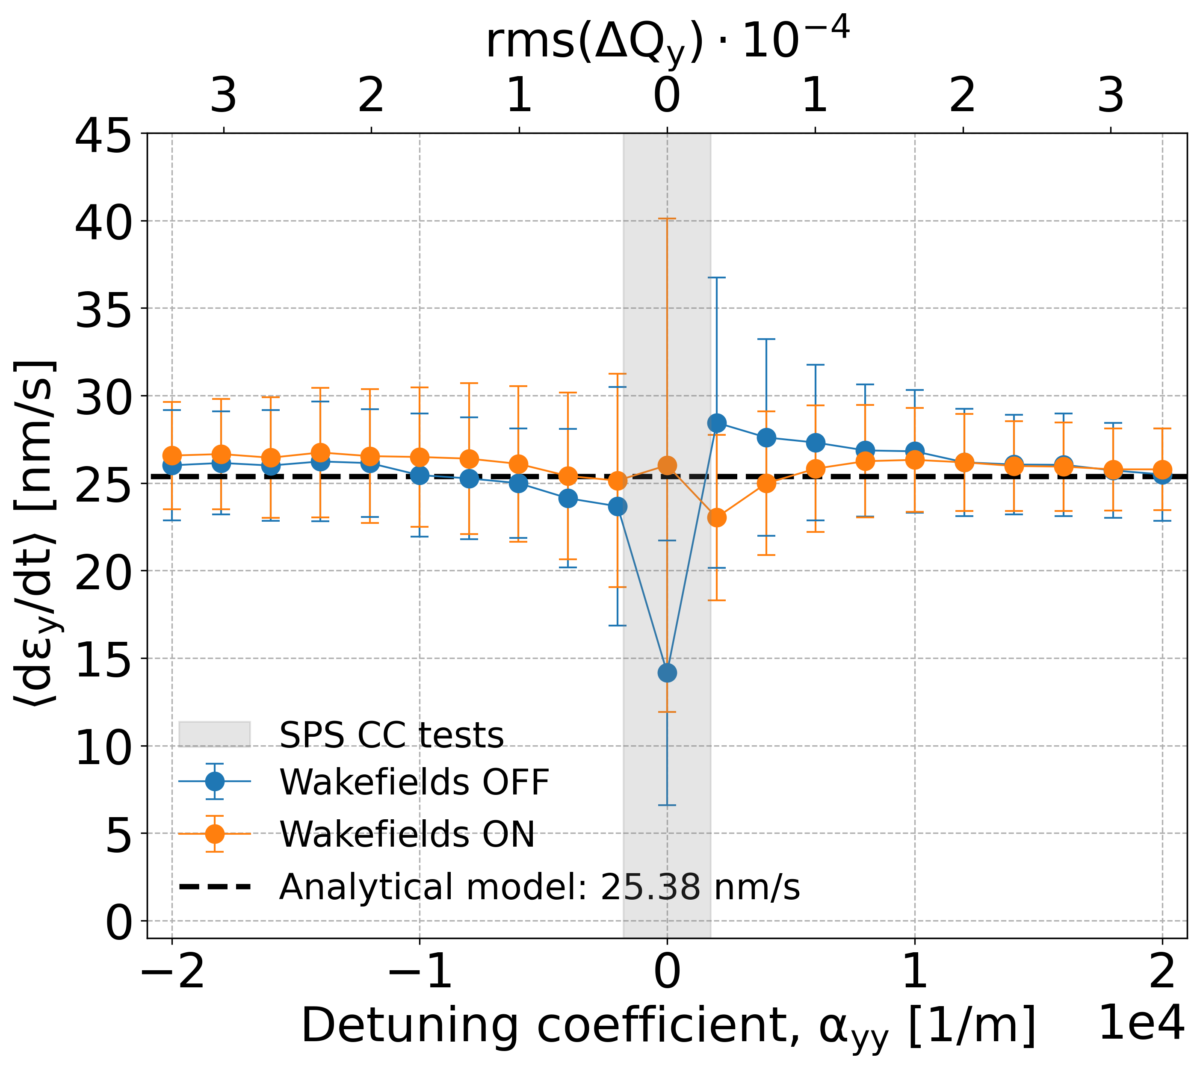
\includegraphics[width=.95\linewidth]{images/Ch7/quadrupolar_impedance.png}
        \caption{Only quadrupolar (detuning) impedance contribution.}
        \label{fig:study_7_quad}
    \end{subfigure}
    \begin{subfigure}{.45\textwidth}
        \centering
        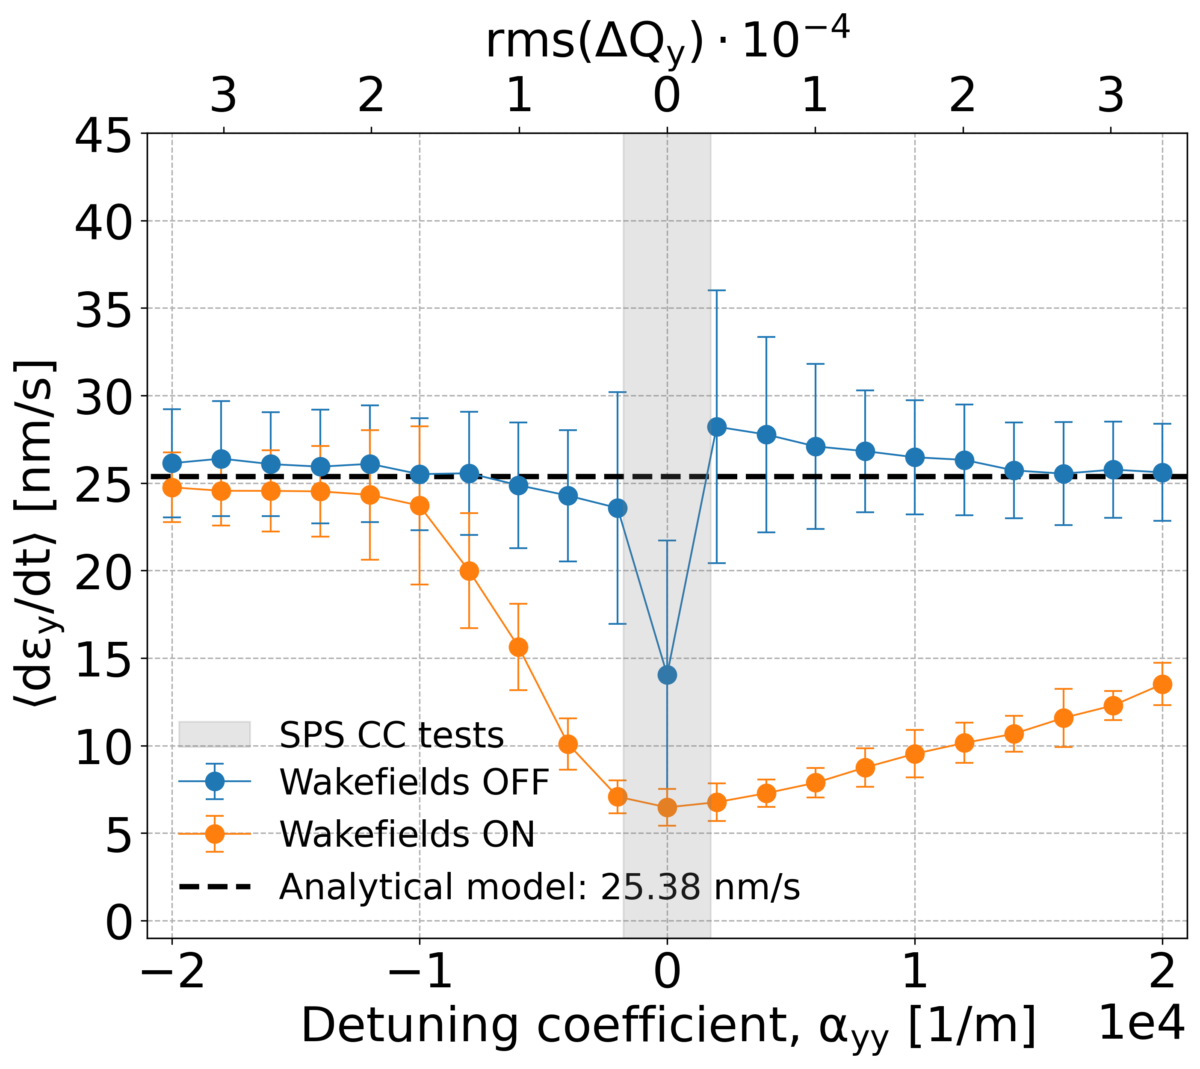
\includegraphics[width=.95\linewidth]{images/Ch7/deyRates_final_2018_PN_sps_270GeV_PN1e-8_400MHz_y-plane_QpxQpy5e-1_6D_Nb5e5_intensity3e10_ayyScan_wakesON_vs_OFF_vs_TuneSpreadvsExpectedSPS.png}  
        \caption{Dipolar (driving) and quadrupolar (detuning) impedance contribution.}
        \label{fig:study_7_dipole_and_quad}
    \end{subfigure}   
    \caption{Transverse emittance growth driven by CC RF phase noise at 400\,MHz without (blue) and with (orange) the impedance effects as a function of tune spread. \textit{Top}: Simulation results with only the dipolar (left) and quadrupolar (right) impedance contribution. \textit{Bottom}: Simulation results with the dipolar and quadrupolar impedance contributions combined.}
    \label{fig:study_7_dipole_vs_quadrupole}
\end{figure}

Looking at the emittance growth rates obtained in the presence of wakefield kicks (orange), it becomes evident that the dipolar contribution (Fig.~\ref{fig:study_7_dipole}) results in a strong suppression of the emittance growth which has the same dependence on the tune spread with the simulations that include both the dipolar and quadrupolar terms. On the contrary, the emittance growth remains unaffected when only the quadrupolar contribution is taken into account (Fig.~\ref{fig:study_7_quad}). Thus, it is evident, that the effect of the suppression is a result of the dipolar term of the impedance. 

The consequence of the dipolar term is that it leads to coherent tune shift (see Section~\ref{subsec:wakefields}). Therefore, these simulation results provide strong evidence that the observed suppression of the noise-induced emittance growth is associated with the coherent tune shift from the dipolar impedance contribution. This suggestion and consequently the mechanism behind the observed suppression will be further explored in the next section.


\section{Suppresion mechanism}\label{sec:suppression_mechanism}
The goal of this section is to understand the mechanism behind the suppression of the emittance growth observed in the presence of the transverse impedance in the SPS case. 

- We return to the first case, in section 7.3
The followinf studies are organised following the observation of the dependece on the coherent tune shift.

\subsection{Historical considerations and motivation}\label{subsec:past_studies_impedance_suppression_BB}
% Or: Past studies with beam-beam interactions

As concluded in Section~\ref{sec:emittance_growth_exploratory_studies}, the effect of the emittance growth suppression from the beam coupling impedance is associated with the coherent tune shift, caused by the dipolar impedance term. This triggered the idea, that overlap between the coherent tune and the incoherent spectrum \footnote{Incoherent spectrum is defined as the set of the oscillation frequencies of the individual particles within a bunch.} could explain the observed effect of the suppression. 
% Or: "This lead to the proposal.." instead of "triggered the idea".

The motivation for this idea came from the fact that past theoretical studies from Y.~Alexahin~\cite{Alexahin:314169} showed that in hadron colliders the efficiency of the feedback system at suppressing the emittance growth depends on the overlap between the frequency of the coherent mode and the incoherent spectrum. In particular, the presence of a coherent mode outside of the incoherent spectrum drastically suppresses the decoherence of the dipole oscillations. This theory has been verified by numerical simulations and experimental studies for LHC~\cite{QIANG201853, PhysRevAccelBeams.23.021002, PhysRevAccelBeams.24.011003}. % The references were taken from p.9: https://indico.cern.ch/event/1170242/contributions/4915101/attachments/2476586/4250387/2022-07-07_crabMD-expanded.pdf
For reference, additional simulation studies for the LHC case which deal with the above-mentioned phenomenon of decoherence suppression can be found in Refs.~\cite{Alexahin:497415, Herr:486007}. 

However, in these studies, the frequency of the coherent modes was shifted by the beam-beam effect \footnote{Beam-beam effects, are the ones induced by the perturbation of the two beams in a collider as they cross each other. Further details on these effects and the beam-beam interaction can be found in Ref.~\cite{Herr:1982430} but their analysis is out of the scope of this thesis.} and not by the beam coupling impedance. Adjusting the theoretical approach of Y.~Alexahin for the impedance-induced tune shift is not straightforward (see section ..). To this end, the strategy that was followed to further explore the mechanism of the emittance growth suppression by the transverse impedance was tracking simulations with PyHEADTAIL. These simualtion studies will be presented and discussed in the following subsections.


\subsection{Intensity scans}\label{subsec:intensity_scan_emit_growth}
To test the hypothesis that the observed suppression of the emittance growth is a result of the separation of the coherent mode from the incoherent spectrum intensity scans were made. As discussed in the Introduction (Section~\ref{subsec:wakefields}) and illustrated in Section~\ref{subsec:test_implementation_pyheatail} the shift of the coherent tune increases (in absolute value) linearly for increasing intensity. Therefore, when simulating the emittance growth in the presence of wakefields over a range of different intensities a cut-off effect should be expected at the moment the frequency of the coherent mode is shifted outside of the incoherent spectrum.

The simulation was performed for the beam and machine conditions of the 2018 $\CC$ experiments in the SPS as shown in Section~\ref{sec:first_obs_suppression}. The $\CC$ RF phase noise kick that was acting on the beam had a power spectral density of 1.68\,$\mathrm{rad^2/Hz}$, which results to about 25\,nm/s. 

In the above-mentioned section, it was shown that in order to reproduce the realistic rms tune spread ($\sim 2-3 \times 10^{-4}$) that was present in SPS during the 2018 experiments (from intrinsic non-linearities), the vertical amplitude detuning coefficient should be $| \alpha_\mathrm{yy} |$=2000\,1/m. However, it becomes evident from Fig.~\ref{fig:MD_2018_impedance_simulations} that this leads to the regime of very strong suppression, which might toughen up this parametric study. Therefore, the intensity scan was performed for $\alpha_\mathrm{yy}$=6000\,1/m which leads to a regime of medium suppression but is still close enough to the realistic machine conditions of 2018.

%To have the clearest visualisation of the effect possible, the emittance growth was induced by a dipolar noise kick (instead of a $\CC$ phase noise kick). The power spectral density of the noise was set to 3.36\,$\mathrm{rad^2/Hz}$ which results to a transverse emittance growth of $\sim$25\,nm/s (see Section~\ref{subsec:dipole_noise}). Furthermore, the vertical amplitude detuning coefficient was set to $\alpha_\mathrm{yy}=6000$\,1/m which corresponds to the regime of strong suppression (see Fig.~\ref{fig:study_5_dipole_noise}). Last, the linear chromaticity was corrected to zero, $Q^\prime_{x,y}$=0, such as it does not introduce any additional tune spread and hence simplify the observables.

% Location: cernbox/pyheadtail_data/final_for_thesis/2018_conditions/study_8_intensity_scans/CCphaseNoise
\begin{figure}[!h] 
    \centering         
    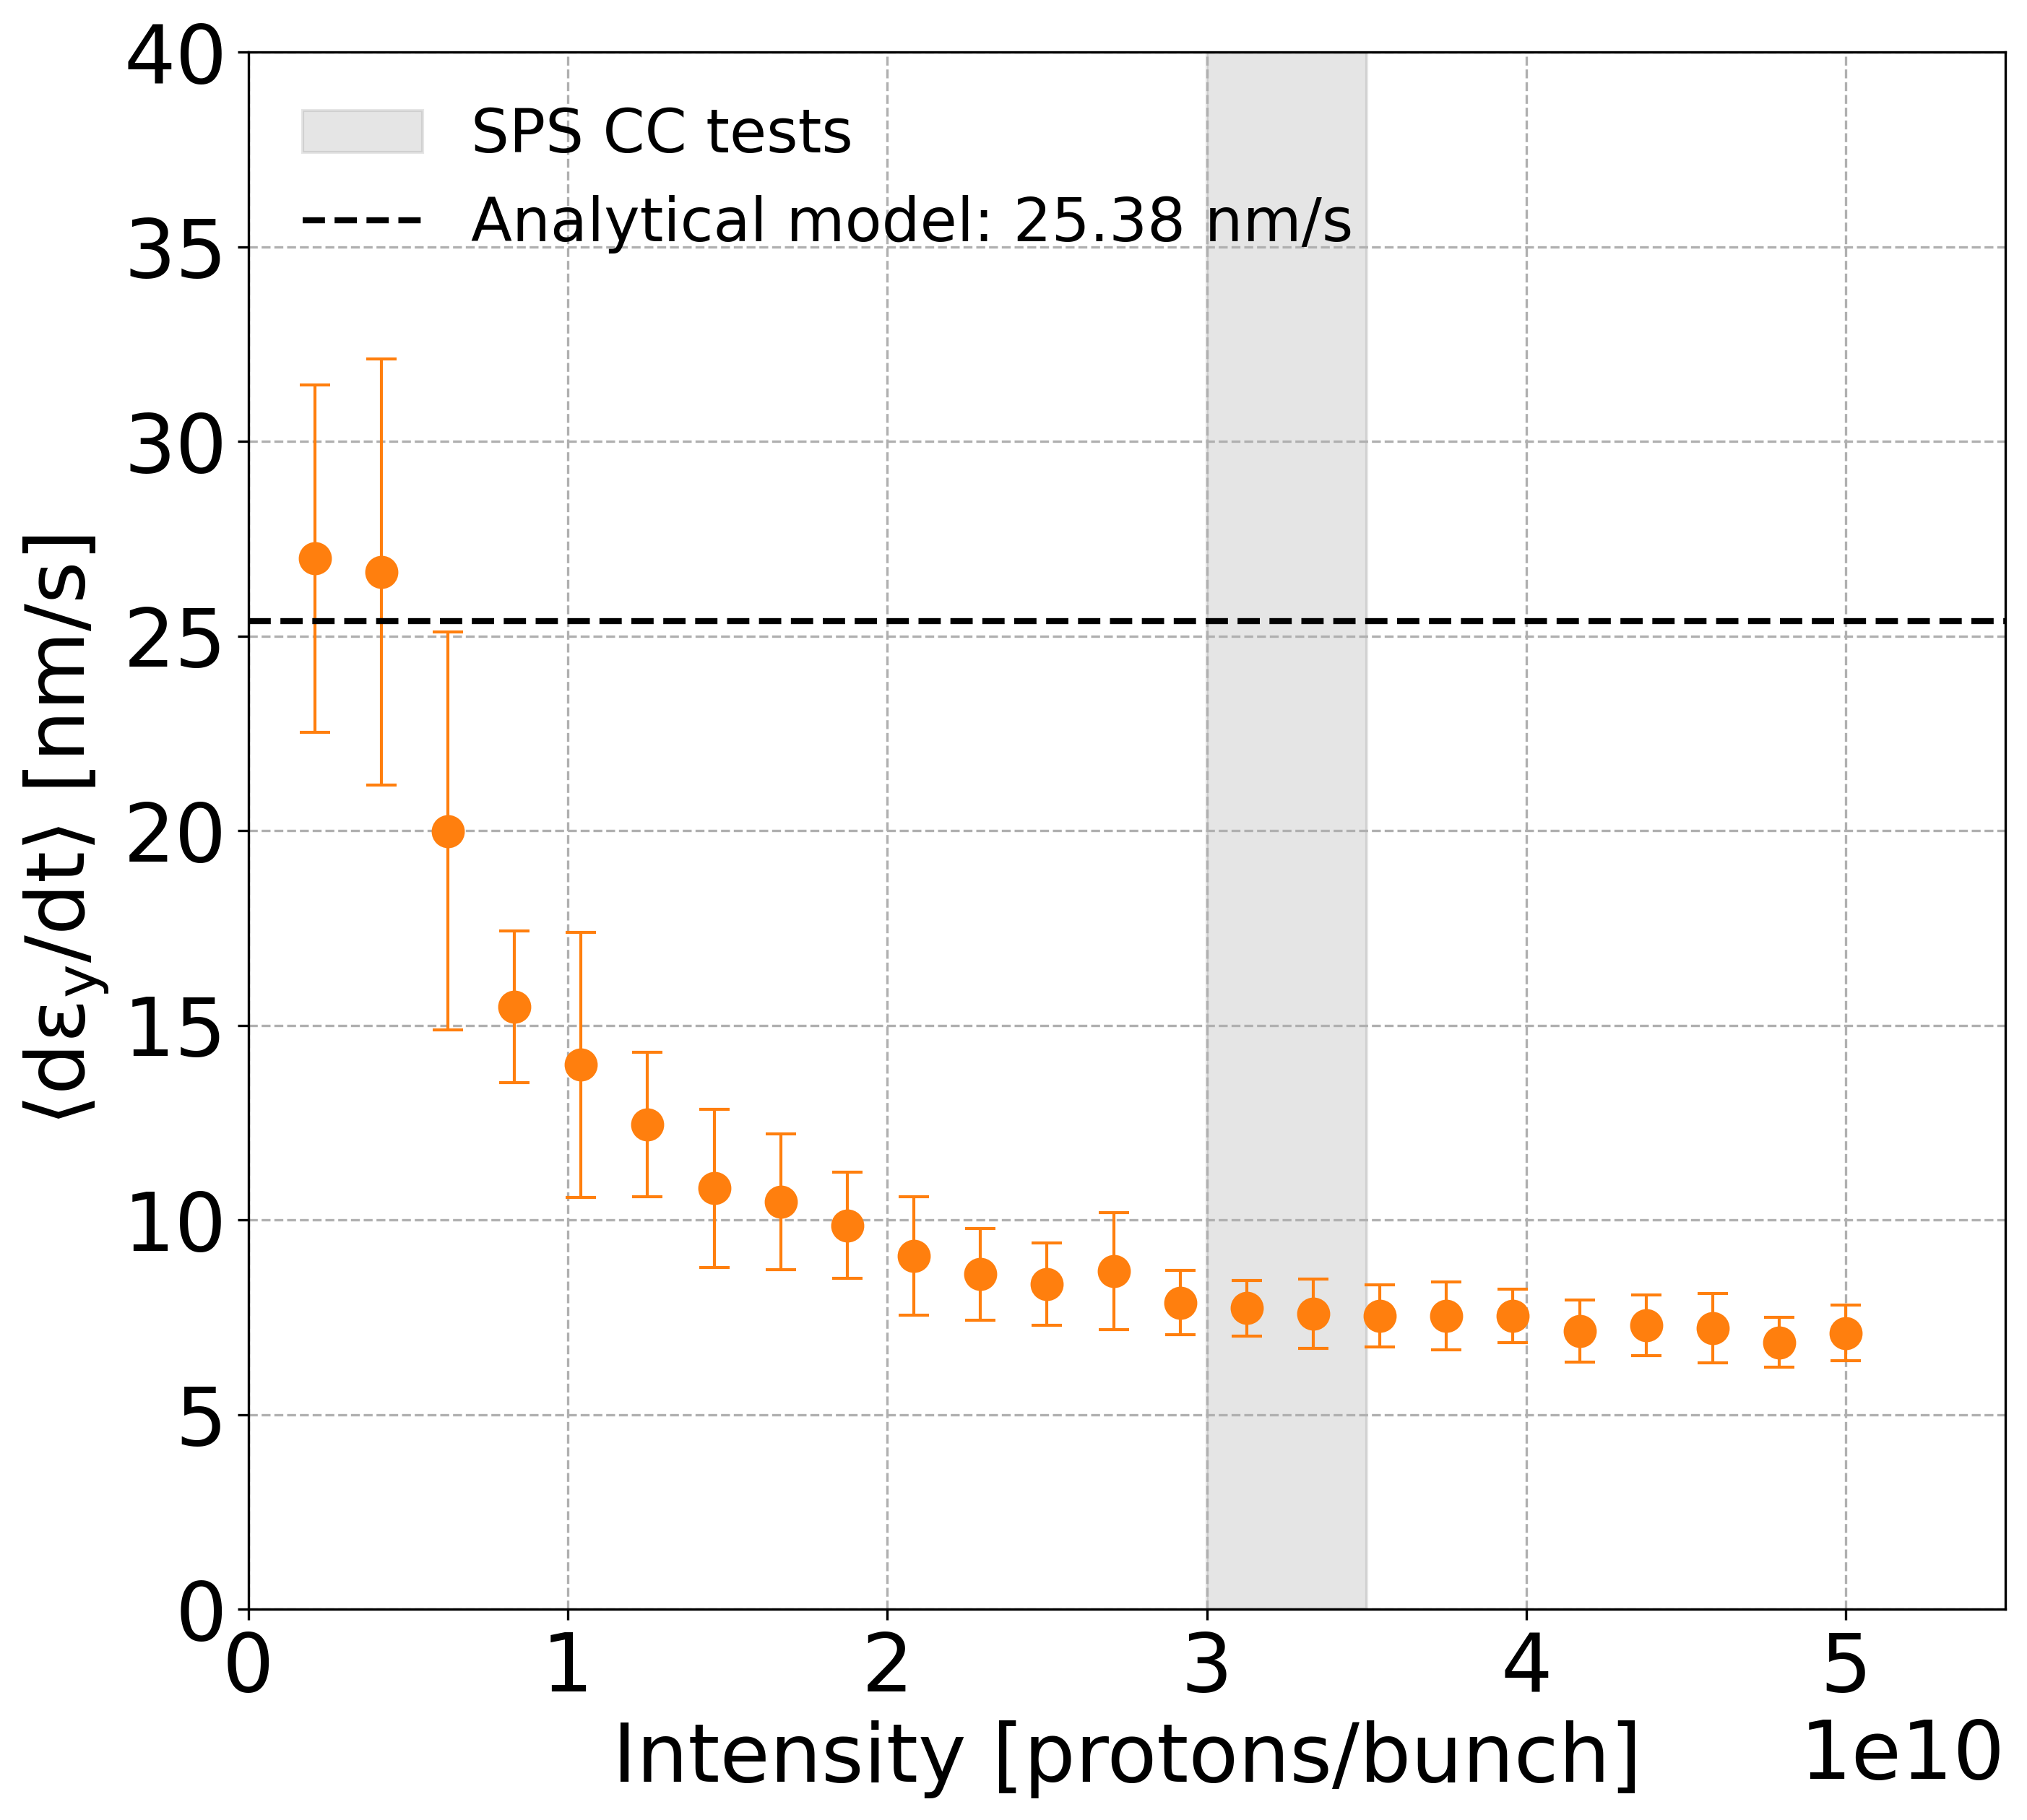
\includegraphics[width=0.7\textwidth]{images/Ch7/sps_270GeV_PN1e-8_400MHz_QpxQpy5e-1_ayy6000_intensity_spsCCtests.png}
        \caption{PyHEADTAIL simulations illustrating the effect of the beam intensity on the transverse emittance growth driven by CC RF phase noise in the presence of impedance effects. The blue vertical line shows the intensity value during the SPS CC tests in 2018.}
        \label{fig:study_8_intensity_scan}
 \end{figure}

 The study was conducted over a range of bunch intensities equally spaced from 0 to $5 \times 10^{10}$ protons per bunch. This range was chosen to be in the vicinity of the $\CC$ experiments in SPS in 2018, where the intensity was $3 \times 10^{10}$ protons per bunch. No simulations were conducted for zero intensity as it is not a realistic value.

 The results of the intensity scan are summarised in Fig.~\ref{fig:study_8_intensity_scan}, where the simulated emittance growth rate is plotted as a function of intensity. The intensity value during the SPS $\CC$ experiment of 2018 is given by the blue vertical line for reference. For small intensity values, $< \sim 0.7\times 10^{10}$ protons, the emittance growth rates appear unaffected from the intensity change and equal $\sim$25\,nm/s as expected. However, for intensity slightly larger than $\sim 0.7 \times 10^{10}$ protons there is a sudden drop in the obtained growth rates. After that point, the growth rates seem to decrease with increasing intensity. This dependence seems to saturate for larger intensity values, $>\sim 2.5 \times 10^{10}$ protons. Last, it becomes evident that the intensity value of the SPS $\CC$ tests (blue line) is well inside the regime of strong suppression.

The important observation of this study is that indeed a cut-off effect appears in the dependence of the simulated emittance growth on the intensity which is a strong indication that the effect of the suppression is indeed associated with the separation of the coherent mode from the incoherent spectrum. To further validate this hypothesis, follow-up simulations were performed aiming to examine the frequency spectrum of the bunch, which should reveal more information on the overlap of the coherent mode frequency and the incoherent spectrum. These simulations will be discussed in the next subsection.



\subsection{Spectral analysis of the bunch centroid motion}\label{subsec:spectral_analysis_schottky}
Here, the incoherent spectrum of the bunch is investigated for different intensities in an attempt to visualise and hence confirm that the suppression mechanism is a result of the separation of the coherent mode from the incoherent spectrum. The incoherent spectrum can be obtained from Fourier's analysis of the turn-by-turn centroid motion. This method can be also found in the bibliography as Schottky noise method~\cite{Caspers:1213284} and is often used for beam diagnostics as it can reveal information on important parameters such as the revolution frequency, the momentum spread, and of course the incoherent spectrum.

For the spectral analysis studies presented here, the simualtions present in the previously, in Subsection~\ref{subsec:intensity_scan_emit_growth} were repeated but without applying any noise kick on the bunch to minimise the external perturbations and obtain a clear frequency signal. This choice is justified since the noise kicks do not have any impact on the frequency domain. Additionally, now the six-dimensional Gaussian bunch distribution was generated with an initial vertical offset of 0.2 times the vertical beam size. The reason behind this is that due to the offset the beam will undergo betatron oscillations with a higher amplitude which will facilitate the Fourier analysis. Furthermore, this type of simulation requires longer tracking than the emittance growth studies, $10^6$ turns instead of $10^5$, for better representation in the frequency domain. Last, $5 \times 10^4$ macroparticles were sufficient \footnote{Following similar studies in Ref.~\cite{Zorzano-Mier:446334} and exploratory studies confirmed that the number of macroparticles used does not affect the quality of the results.} for this type of simulation which reduced significantly the computational time of the simulation. 

The spectra that will be discussed below were obtained by applying a NAFF algorithm to the turn-by-turn data as described in Section~\ref{subsec:test_implementation_pyheatail}. Last, the amplitude of the spectral components is expressed as power spectral density in units of $\mathrm{rad^2}/Q_y$ as it is preferred over the amplitude of the spectral components of the Fourier transform which is in arbitrary units. The power spectral density of the motion of the centroid is obtained from the above-mentioned Fourier transform using Eq.~\eqref{eq:Sxx_definition_discrete_normalized}.

The results are displayed in Fig.~\ref{fig:study_9_schottky_noise_intnensity_scan} which shows the vertical spectrum of the centroid (coherent) oscillation of the bunch for different intensity values, selected from the range studied in the previous Subsection~\ref{subsec:intensity_scan_emit_growth}, such as the separation of the coherent tune form the incoherent spectrum is clearly visible. Each subplot shows the power spectral density of the motion of the centroid as a function of the frequency in tune units for a given intensity value, which increases from the top left to the bottom right. The frequency of the coherent mode is shown with the vertical magenta line and it corresponds to the frequency with the highest amplitude.

% cernbox: /pyheadtail_data/final_for_thesis/2018_conditions/study_9_schottky_noise_spectra/QpxQpy5e-1/
 \begin{figure}[htp]
    \centering
    \begin{subfigure}{.45\textwidth}
        \centering
        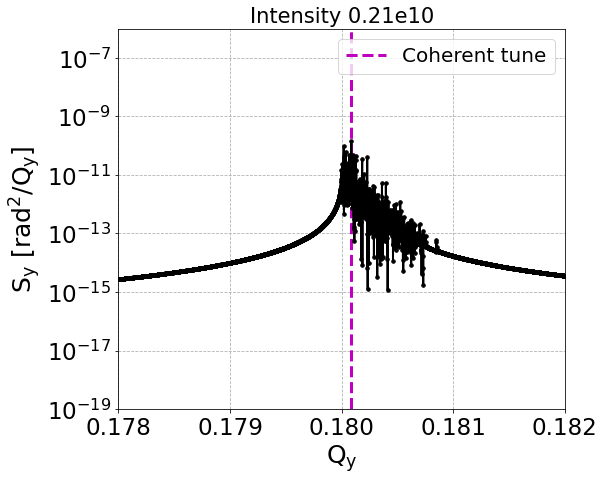
\includegraphics[width=.95\linewidth]{images/Ch7/psdY_intensity0.21e10.png}  
        %\caption{$Q^\prime_{x,y}$=0.0}
        \label{fig:study_9a}
    \end{subfigure}
    \begin{subfigure}{.45\textwidth}
        \centering
        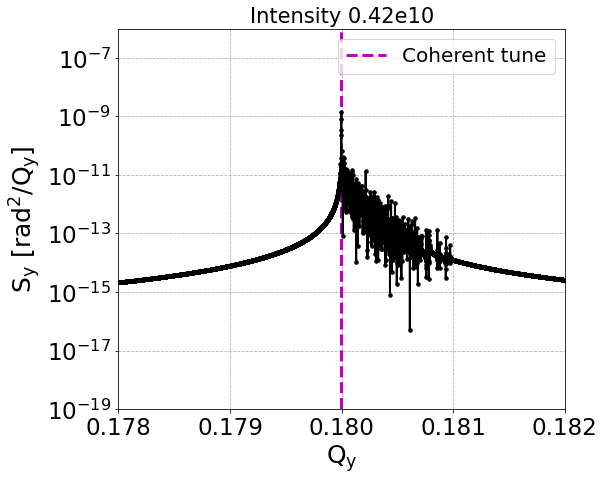
\includegraphics[width=.95\linewidth]{images/Ch7/psdY_intensity0.42e10.png}
        %\caption{$Q^\prime_{x,y}$=0.5}
        \label{fig:study_9b}
    \end{subfigure}
    \begin{subfigure}{.45\textwidth}
        \centering
        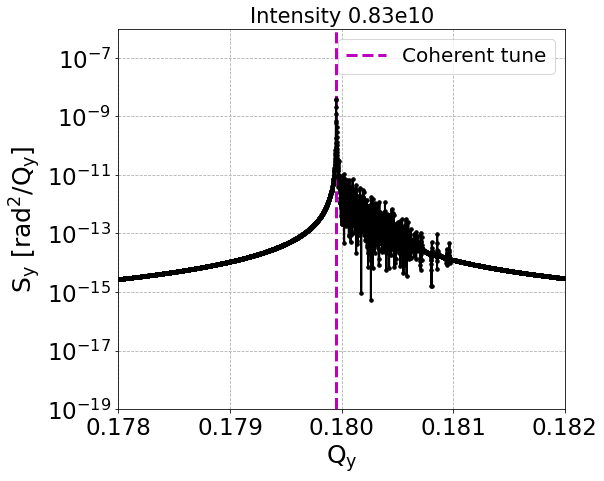
\includegraphics[width=.95\linewidth]{images/Ch7/psdY_intensity0.83e10.png}  
        %\caption{$Q^\prime_{x,y}$=1.0}
        \label{fig:study_9c}
    \end{subfigure}
    \begin{subfigure}{.45\textwidth}
        \centering
        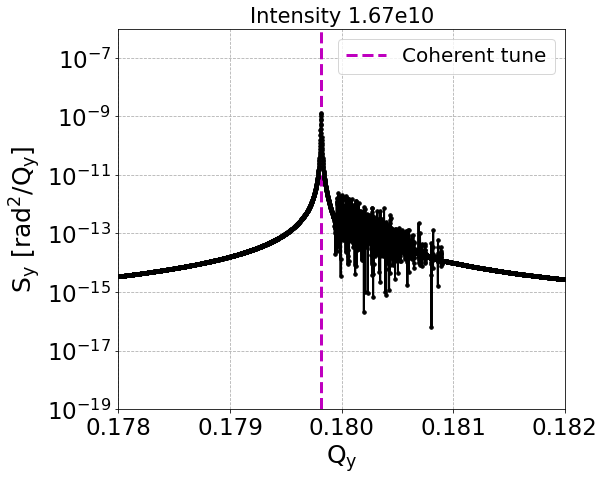
\includegraphics[width=.95\linewidth]{images/Ch7/psdY_intensity1.67e10.png}  
        %\caption{$Q^\prime_{x,y}$=2.5}
        \label{fig:study_9d}
    \end{subfigure}
    \begin{subfigure}{.45\textwidth}
        \centering
        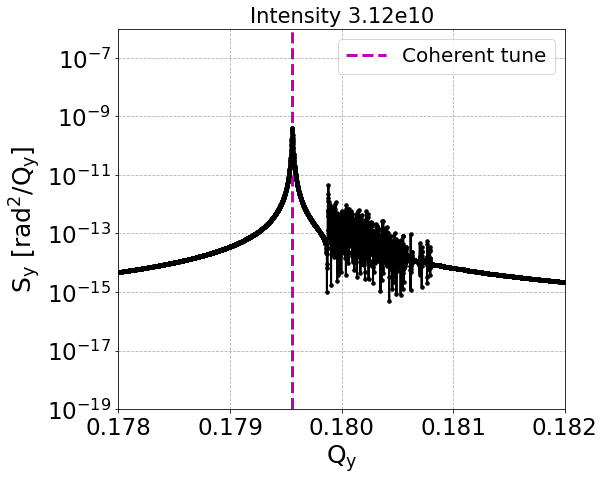
\includegraphics[width=.95\linewidth]{images/Ch7/psdY_intensity3.12e10.png}  
        %\caption{$Q^\prime_{x,y}$=5.0}
        \label{fig:study_9e}
    \end{subfigure}
    \begin{subfigure}{.45\textwidth}
            \centering
            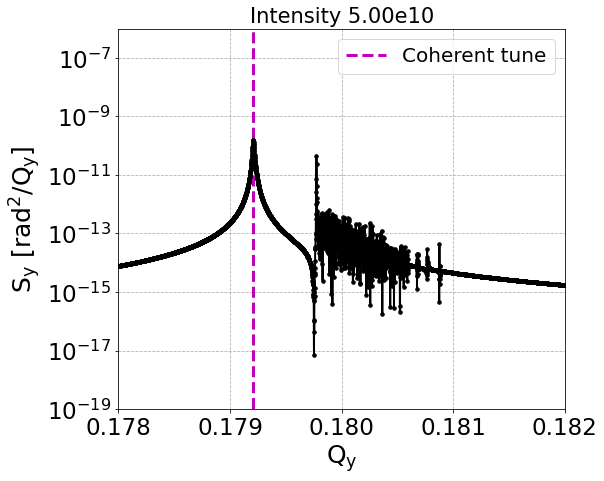
\includegraphics[width=.95\linewidth]{images/Ch7/psdY_intensity5.00e10.png}  
            %\caption{$Q^\prime_{x,y}$=2.5}
            \label{fig:study_9f}
    \end{subfigure}
    \caption{Power spectral density of the vertical bunch centroid motion on a logarithmic scale in the presence of the SPS transverse impedance model, calculated over $10^6$ turns with $5 \times 10^4$ macroparticles for different values of intensity increasing from top left to bottom right.}
    \label{fig:study_9_schottky_noise_intnensity_scan}
\end{figure}

Comparing Fig.~\ref{fig:study_9_schottky_noise_intnensity_scan} with Fig.~\ref{fig:study_8_intensity_scan} it becomes evident that:
\begin{itemize}
    \item The two upper spectra, where the coherent mode lies inside the incoherent spectrum, reside in the regime of no emittance growth suppression.
    \item The two middle spectra, where the coherent mode emerges from the incoherent spectrum, reside in the regime where the emittance growth suppression increases for higher intensity values.
    \item The two bottom spectra, where the cohere mode is well separated from the incoherent spectra, reside in the regime where the dependence on the intensity saturates.
\end{itemize}

The above observations, confirm that the transverse impedance separates the coherent tune from the incoherent spectrum and this is the mechanism that leads to an effective suppression of the Crab Cavity phase noise induced emittance growth.

According, to Y.~Alexahin's theory for beam-beam induced effects, the explanation is that only part of the energy from the noise kicks is absorbed by the incoherent spectrum and drives incoherent motion and leads to irreversible emittance growth. The rest of the energy is absorbed by the coherent mode, which is damped \footnote{The damping rate of the coherent tune (mode 0) for the experimental parameters of 2018, was estimated to be 3.6 1/turns using Eq.~\eqref{eq:imaginary_tune_mode_l}} by the impedance (for the expereimental conditions of small positve chromaticity) without leading to emittance growth.
% From IPAC's presentation.
% Compute tune shift and damping rate from impedance: https://github.com/natriant/exploring_SPS/tree/master/tuneShift_from_transverese_impedance/theoretical%20model%20(Chao%20formula).

%- he separation of the coherent modes and the incoherent spectrum means that the interaction between the coherent mode and the incoherent motion of the single particles is reduced , source:% https://docs.google.com/presentation/d/1D4WODJEieOKkYta2Oh1h7AN2drb0ti1R-iTjDkwZo6A/edit#slide=id.gca25e861ba_0_170


\subsection{Studying the motion of the centroid - decoherence}
% google slides presentation: https://docs.google.com/presentation/d/1ksIQEaxE5FoVOY7oTd7lwEuIt8P9K3u4lQtENXmD-T4/edit#slide=id.gb54efd84b7_0_0
According to the studies of Y.~Alexahin (which were performed in the context of the beam-beam modes) the separation of the coherent mode from the incoherent spectrum results in a suppression of the decoherence of the dipole oscillations and thus of the dipole and/or phase-noise-induced emittance growth. 


This section is dedicated in visualising the change in the decoherence and the associated transverse emittance growth 


In this subsection, the decoherence and the associated transverse emittance growth are simulated with PyHEADTAIL with and without the impact of the wakefields for different intensity and chromaticity values. The objective of the study is to demonstrate the above mentioned changes in the decoherence due to the coherent tune shift but introduced by the beam coupling imepdance instead of the beam-beam effects.

illustrate the changes in the decoherence and thus in the emittance growth during the 

PyHEADTAIL tracking simualtions 


the suppression is a results of the change in decohernce (|see how you wirte it in the ipc paper)
this is what is studied here.

PyHEADTAIL simulations of the evolution of the centroid vs emittance for difference values os amplitude detuning. 

\subsection{Dependence on bunch length}
% Slides for the respective studies: 
% https://docs.google.com/presentation/d/1RZ9yE5tAIyGtRutjMaDiJG0t-a1KDnBX1sMgy__wUfM/edit#slide=id.gcbdbf59062_0_68

In this section, the sensitivity of the emittance growth in the presence of $\CC$ RF phase noise and impedance is studied as a function of the bunch length. The goal of this study is a) to complete the set of parametric studies presented already in this chapter and b) to identify possible limitations on observing the effect of the suppression introduced by the bunch length. The latter is very important for the second experimental campaign with $\CC$s in the SPS that took place in early 2022 and will be discussed in further detail in the following chapter.

This parametric study was conducted for the experimental beam and machine conditions of 2018 which are also reported in Tables~\ref{tab:pyheadtail_simulation_parameters} and~\ref{tab:CC_pyheadtail_simulation_parameters} and as shown in Section~\ref{sec:first_obs_suppression}. The $\CC$ RF phase noise kick that was acting on the beam had a power spectral density of 1.68\,$\mathrm{rad^2/Hz}$, which results to about 25\,nm/s. The vertical amplitude detuning coefficient was  $\alpha_\mathrm{yy}$=2000\,1/m in order to reproduce the realistic rms tune spread ($\sim 2-3 \times 10^{-4}$) that was present in SPS during the 2018 experiments (from intrinsic non-linearities). The study was performed over a range of rms bunch lengths equally spaced from 0 to 4\,ns (this refers to 4$\sigma_t$). In practice no simualtions were conducted for zero bunch length as it is not a realistic value.


The study is repeated with and without including the effect of the wakefields for comparison. The PyHEADTAIL simulation results are summarised in Fig.~\ref{fig:study_10_bunch_length} along with the predictions of the theoretical model of T.~Mastoridis and P.~Baudrenghien which doesn't include the impedance effects for completeness.

\begin{figure}[!h] % cernbox/=/pyheadtail_data/final_for_thesis/2018_conditions/study_5_dipole_nois
    \centering         
    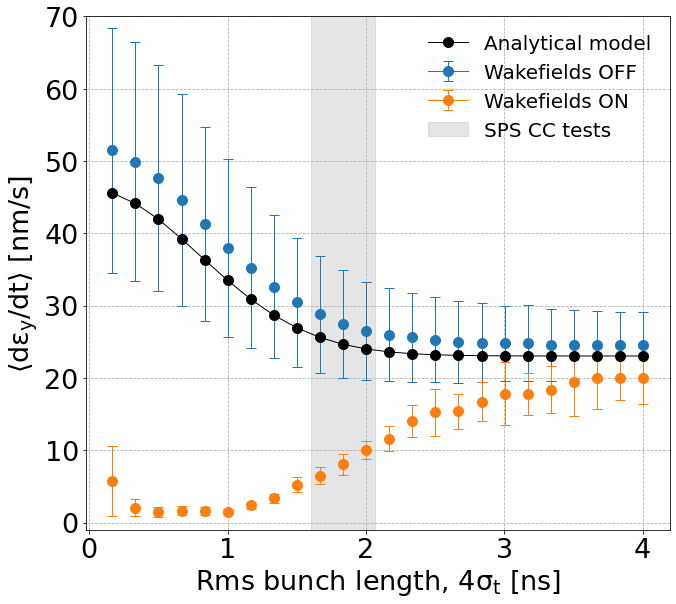
\includegraphics[width=0.7\textwidth]{images/Ch7/deyRates_sps_PN1e-8_00MHz_270GeV_wakesOFF_vs_ON_QpxQpy5e-1_Nb5e5_ayy2000_slices500_intensity3e10_sigmaScanScanZvsTheorywithoutWakes_vs_SPS_sigmaz_ignore_first_point.png}
        \caption{PyHEADTAIL simulations illustrating the effect of the bunch length on the transverse emittance growth driven by CC RF phase noise in the absence (blue) and in the presence (orange)of impedance effects. The analytical predicted growth rates (not including impedance effects) are also shown (black). The regime of the realistic bunch length values during the SPS CC tests of 2018 is depicted with the grey stripe.}
        \label{fig:study_10_bunch_length}
 \end{figure}

 Figure~\ref{fig:study_10_bunch_length} illustrates, as expected, that the simulation results without the wakefields (blue) are in very good agreement with the theoretical predictions (black model), within the error bars. In the presence of wakefields (orange) there is a clear sensitivity of the obtained emittance growth and thus on the suppression from the beam coupling impedance on the rms bunch length. In particular for bunch length values smaller than 1\,ns the suppression appears very strong and it is also independent from the bunch length value. For longer bunches, up to about 3.5\,ns ($\mathrm{4 \sigma_t}$) the suppression factor appears to decrease with the bunch length. For bunches longer than 3.5\,ns ($\mathrm{4 \sigma_t}$) the dependence of the obtained emittance growth on the bunch length seems to saturate. The rates are also in agreement with the theoretical model which does not include the contribution from the wakes. The behavior of the dependence, which is inversely proportional to the bunch length value is explained by the fact that the coherent tune shift from the impedance is also inversely proportional to the bunch length. In other words, for small bunches the coherent tune shift from the impedance is strong and thus the coherent mode emerges from the incoherent spectrum leading to the strong emittance growth suppression. For larger bunch lengths the shift of the coherent mode is weaker resulting in weaker suppression which eventually saturates once the coherent mode lies inside the incoherent spectrum.

 Last, it should be noted that for very small bunches the wake potential used for the simulations may not approximate well the wake function. This seems to be the reason that the first point of the simulation results with the wakefields seems to not follow the otherwise smooth dependence on the bunch length. This appears to be the lower bunch length limit that we can trust the simulations.


% Maybe comment on the experiment.


\section{Conclusions}\label{sec:Ch7_conclusions}
PyHEADTAIL simulations showed for the first time that the transverse beam impedance (not included in the theory nor in the numerical simulations so far) has a significant impact on the emittance growth. In particular, it was found that the transverse impedance can suppress the crab cavity noise-induced emittance growth once the coherent tune, which is shifted by the impedance, moves out of the incoherent tune spectrum. It turns out that the decoherence process is slowed down and thus the noise-induced emittance growth is suppressed. This mechanism, which has been observed in the past as a result of beam-beam interactions, is related to the transverse dipole oscillation of the beam. To this end, the suppression is not observed for amplitude but only for phase noise-induced emittance growth.

For the beam and machine conditions as in the 2018 SPS experiment, the simulations with the complete SPS transverse impedance model revealed a strong suppression of about a factor 4-5 which agrees with the experimental observations and hence it appears to explain the observed discrepancy with the theoretical model of T.~Mastoridis and P.~Baudrenghien (see Chapter~\ref{Ch:2018_analyisis}). 

The PyHEADTAIL simulations also revealed a strong sensitivity of the suppression factor to the amplitude-dependent tune shift. This behavior is very important as it can be tested in the SPS with the use of the Landau octupoles. Based on this, a proof-of-concept experiment was planned and took place in the SPS in 2022, aiming to reproduce the dependence of the emittance growth suppression on the amplitude detuning. Further details and the results of this additional experimental campaign with $\CC$s in the SPS are presented in the next chapter.




